\documentclass[aspectratio=43]{beamer}

% Title --------------------------------------------
\title{\huge The state, the nation, and war}
\author{Francisco Villamil}
\date{War, peace, and political violence\\UC3M, Fall 2023}

%%% NOTE -- CHECK THIS: https://github.com/paulgp/beamer-tips


%%% Building heavily on https://github.com/kylebutts/templates

% xcolor, define them
\usepackage{xcolor}

% TEXT COLORS
\definecolor{red}{HTML}{9a2515}
\definecolor{yellow}{HTML}{EBC944}
\definecolor{asher}{HTML}{555F61}
\definecolor{jet}{HTML}{131516}

% THEME COLORS
\definecolor{accent}{HTML}{107895}
\definecolor{accent2}{HTML}{9a2515}

% Color commands
\newcommand\red[1]{{\color{red}#1}}
\newcommand\yellow[1]{{\color{yellow}#1}}
\newcommand\asher[1]{{\color{asher}#1}}

\newcommand\BGred[1]{{\colorbox{red!80!white}{#1}}}
\newcommand\BGyellow[1]{{\colorbox{yellow!80!white}{#1}}}
\newcommand\BGasher[1]{{\colorbox{asher!80!white}{#1}}}

\renewcommand<>{\BGyellow}[1]{\only#2{\beameroriginal{\BGyellow}}{#1}}

% Appendix numbering
\usepackage{appendixnumberbeamer}

% Beamer Options -------------------------------------

% Background
\setbeamercolor{background canvas}{bg = white}

% Change text margins
\setbeamersize{text margin left = 25pt, text margin right = 15pt}

% \alert
\setbeamercolor{alerted text}{fg = accent2}

% Frame title
\setbeamercolor{frametitle}{bg = white, fg = jet}
\setbeamercolor{framesubtitle}{bg = white, fg = accent}
\setbeamerfont{framesubtitle}{size = \small, shape = \itshape}

% Block
\setbeamercolor{block title}{fg = white, bg = accent2}
\setbeamercolor{block body}{fg = jet, bg = jet!10!white}

% Title page
\setbeamercolor{title}{fg = jet}
\setbeamercolor{subtitle}{fg = accent}

%% Custom \maketitle and \titlepage
\setbeamertemplate{title page}
{
    \begin{centering}
      % \vspace{20mm}
      {\Large \usebeamerfont{title}\usebeamercolor[fg]{title}\inserttitle}\\ \vskip0.25em%
      \ifx\insertsubtitle\@empty%
      \else%
        {\usebeamerfont{subtitle}\usebeamercolor[fg]{subtitle}\insertsubtitle\par}%
      \fi%
      {\vspace{10mm}\insertauthor}\\
      \ifx\insertinstitute\@empty%
      \else%
        {\vspace{5mm}\color{asher}\scriptsize{\insertinstitute}}
      \fi%
      {\color{asher}\small{\insertdate}}\\
    \end{centering}
}

% Table of Contents
\setbeamercolor{section in toc}{fg = accent!70!jet}
\setbeamercolor{subsection in toc}{fg = jet}

% Button
\setbeamercolor{button}{bg = accent}

% Remove navigation symbols
\setbeamertemplate{navigation symbols}{}

% Table and Figure captions
\setbeamercolor{caption}{fg=jet!70!white}
\setbeamercolor{caption name}{fg=jet}
\setbeamerfont{caption name}{shape = \itshape}

% Put slide number / total slides at the bottom right
\makeatother
\makeatletter
\setbeamertemplate{footline} %{\hfill\insertframenumber/\inserttotalframenumber}
{%
  \leavevmode%
  \hbox{
  \begin{beamercolorbox}[wd=\paperwidth,ht=2.5ex,dp=1.125ex,leftskip=.3cm,rightskip=.3cm plus1fil]{footlinecolor}%
    \color{asher}{\hfill\insertframenumber/\inserttotalframenumber}
  \end{beamercolorbox}}%
  \vskip0pt%
}
\makeatother
\makeatletter

% Bullet points

%% Fix left-margins
\settowidth{\leftmargini}{\usebeamertemplate{itemize item}}
\addtolength{\leftmargini}{\labelsep}

%% enumerate item color
\setbeamercolor{enumerate item}{fg = accent}
\setbeamerfont{enumerate item}{size = \small}
\setbeamertemplate{enumerate item}{\insertenumlabel.}

%% itemize
\setbeamercolor{itemize item}{fg = accent!70!white}
\setbeamerfont{itemize item}{size = \small}
\setbeamertemplate{itemize item}[circle]
\setlength{\itemsep}{0pt plus 6pt}

%% right arrow for subitems
\setbeamercolor{itemize subitem}{fg = accent!60!white}
\setbeamerfont{itemize subitem}{size = \small}
\setbeamertemplate{itemize subitem}{$\rightarrow$}

\setbeamertemplate{itemize subsubitem}[square]
\setbeamercolor{itemize subsubitem}{fg = jet}
\setbeamerfont{itemize subsubitem}{size = \small}

% References

%% Bibliography Font, roughly matching aea
\setbeamerfont{bibliography item}{size = \footnotesize}
\setbeamerfont{bibliography entry author}{size = \footnotesize, series = \bfseries}
\setbeamerfont{bibliography entry title}{size = \footnotesize}
\setbeamerfont{bibliography entry location}{size = \footnotesize, shape = \itshape}
\setbeamerfont{bibliography entry note}{size = \footnotesize}

\setbeamercolor{bibliography item}{fg = jet}
\setbeamercolor{bibliography entry author}{fg = accent!60!jet}
\setbeamercolor{bibliography entry title}{fg = jet}
\setbeamercolor{bibliography entry location}{fg = jet}
\setbeamercolor{bibliography entry note}{fg = jet}

%% Remove bibliography symbol in slides
\setbeamertemplate{bibliography item}{}





% Links ----------------------------------------------

\usepackage{hyperref}
\hypersetup{
  colorlinks = true,
  linkcolor = accent,
  filecolor = accent,
  urlcolor = accent,
  citecolor = accent,
}


% Line spacing --------------------------------------
\usepackage{setspace}
\setstretch{1.2}


% \begin{columns} -----------------------------------
\usepackage{multicol}


% % Fonts ---------------------------------------------
% % Beamer Option to use custom fonts
% \usefonttheme{professionalfonts}
%
% % \usepackage[utopia, smallerops, varg]{newtxmath}
% % \usepackage{utopia}
% \usepackage[sfdefault,light]{roboto}
%
% % Small adjustments to text kerning
% \usepackage{microtype}



% Remove annoying over-full box warnings -----------
\vfuzz2pt
\hfuzz2pt


% Table of Contents with Sections
\setbeamerfont{myTOC}{series=\bfseries, size=\Large}
\AtBeginSection[]{
        \frame{
            \frametitle{Roadmap}
            \tableofcontents[current]
        }
    }


% References ----------------------------------------
\usepackage[
    citestyle= authoryear,
    style = authoryear,
    natbib = true,
    backend = biber
]{biblatex}

% Smaller font-size for references
\renewcommand*{\bibfont}{\small}

% Remove "In:"
\renewbibmacro{in:}{}

% Color citations for slides
\newenvironment{citecolor}
    {\footnotesize\begin{color}{accent2}}
    {\end{color}}

\newcommand{\citetcolor}[1]{{\footnotesize\textcolor{asher}{\citet{#1}}}}
\newcommand{\citepcolor}[1]{{\footnotesize\textcolor{asher}{\citep{#1}}}}

% Tables -------------------------------------------
% Tables too big
% \begin{adjustbox}{width = 1.2\textwidth, center}
\usepackage{adjustbox}
\usepackage{array}
\usepackage{threeparttable, booktabs, adjustbox}

% Fix \input with tables
% \input fails when \\ is at end of external .tex file

\makeatletter
\let\input\@@input
\makeatother

% Tables too narrow
% \begin{tabularx}{\linewidth}{cols}
% col-types: X - center, L - left, R -right
% Relative scale: >{\hsize=.8\hsize}X/L/R
\usepackage{tabularx}
\newcolumntype{L}{>{\raggedright\arraybackslash}X}
\newcolumntype{R}{>{\raggedleft\arraybackslash}X}
\newcolumntype{C}{>{\centering\arraybackslash}X}

% Figures

% \imageframe{img_name} -----------------------------
% from https://github.com/mattjetwell/cousteau
\newcommand{\imageframe}[1]{%
    \begin{frame}[plain]
        \begin{tikzpicture}[remember picture, overlay]
            \node[at = (current page.center), xshift = 0cm] (cover) {%
                \includegraphics[keepaspectratio, width=\paperwidth, height=\paperheight]{#1}
            };
        \end{tikzpicture}
    \end{frame}%
}

% subfigures
\usepackage{subfigure}


% Highlight slide -----------------------------------
% \begin{transitionframe} Text \end{transitionframe}
% from paulgp's beamer tips
\newenvironment{transitionframe}{
    \setbeamercolor{background canvas}{bg=accent!60!black}
    \begin{frame}\color{accent!10!white}\LARGE\centering
}{
    \end{frame}
}


% Table Highlighting --------------------------------
% Create top-left and bottom-right markets in tabular cells with a unique matching id and these commands will outline those cells
\usepackage[beamer,customcolors]{hf-tikz}
\usetikzlibrary{calc}
\usetikzlibrary{fit,shapes.misc}

% To set the hypothesis highlighting boxes red.
\newcommand\marktopleft[1]{%
    \tikz[overlay,remember picture]
        \node (marker-#1-a) at (0,1.5ex) {};%
}
\newcommand\markbottomright[1]{%
    \tikz[overlay,remember picture]
        \node (marker-#1-b) at (0,0) {};%
    \tikz[accent!80!jet, ultra thick, overlay, remember picture, inner sep=4pt]
        \node[draw, rectangle, fit=(marker-#1-a.center) (marker-#1-b.center)] {};%
}



\begin{document}

\begin{frame}
  \titlepage
\end{frame}

% ----------------------------------------------------
\begin{frame}
\frametitle{Overview}
\centering

\begin{itemize}
  \item Political violence from a historical view
  \item Two main events deeply connected to violence and war:
  \item<2->[1.] The rise of the \BGyellow{modern state}
  \begin{itemize}
    \item role of violence in the process of state-building
    \item and how wars changed when modern states emerged
  \end{itemize}
  \item<3->[2.] The rise of the \BGyellow{nation-state} (more during seminar)
  \begin{itemize}
    \item nationalism changed how and which wars were waged
    \item and role of political violence in shaping nations
  \end{itemize}
\end{itemize}

\end{frame}
% ----------------------------------------------------

% ============================================================
% ============================================================
% STATE-BUILDING
% ============================================================
% ============================================================


\begin{frame}
\frametitle{The state}
\centering

\begin{itemize}
\item What is a state?
\item Max Weber's definition: a state is a political entity that maintains a monopoly on the legitimate use of violence within its own boundaries
\item ``Compulsory political organization''
\end{itemize}

\end{frame}

\begin{frame}
\frametitle{The state as a criminal organization}
\centering

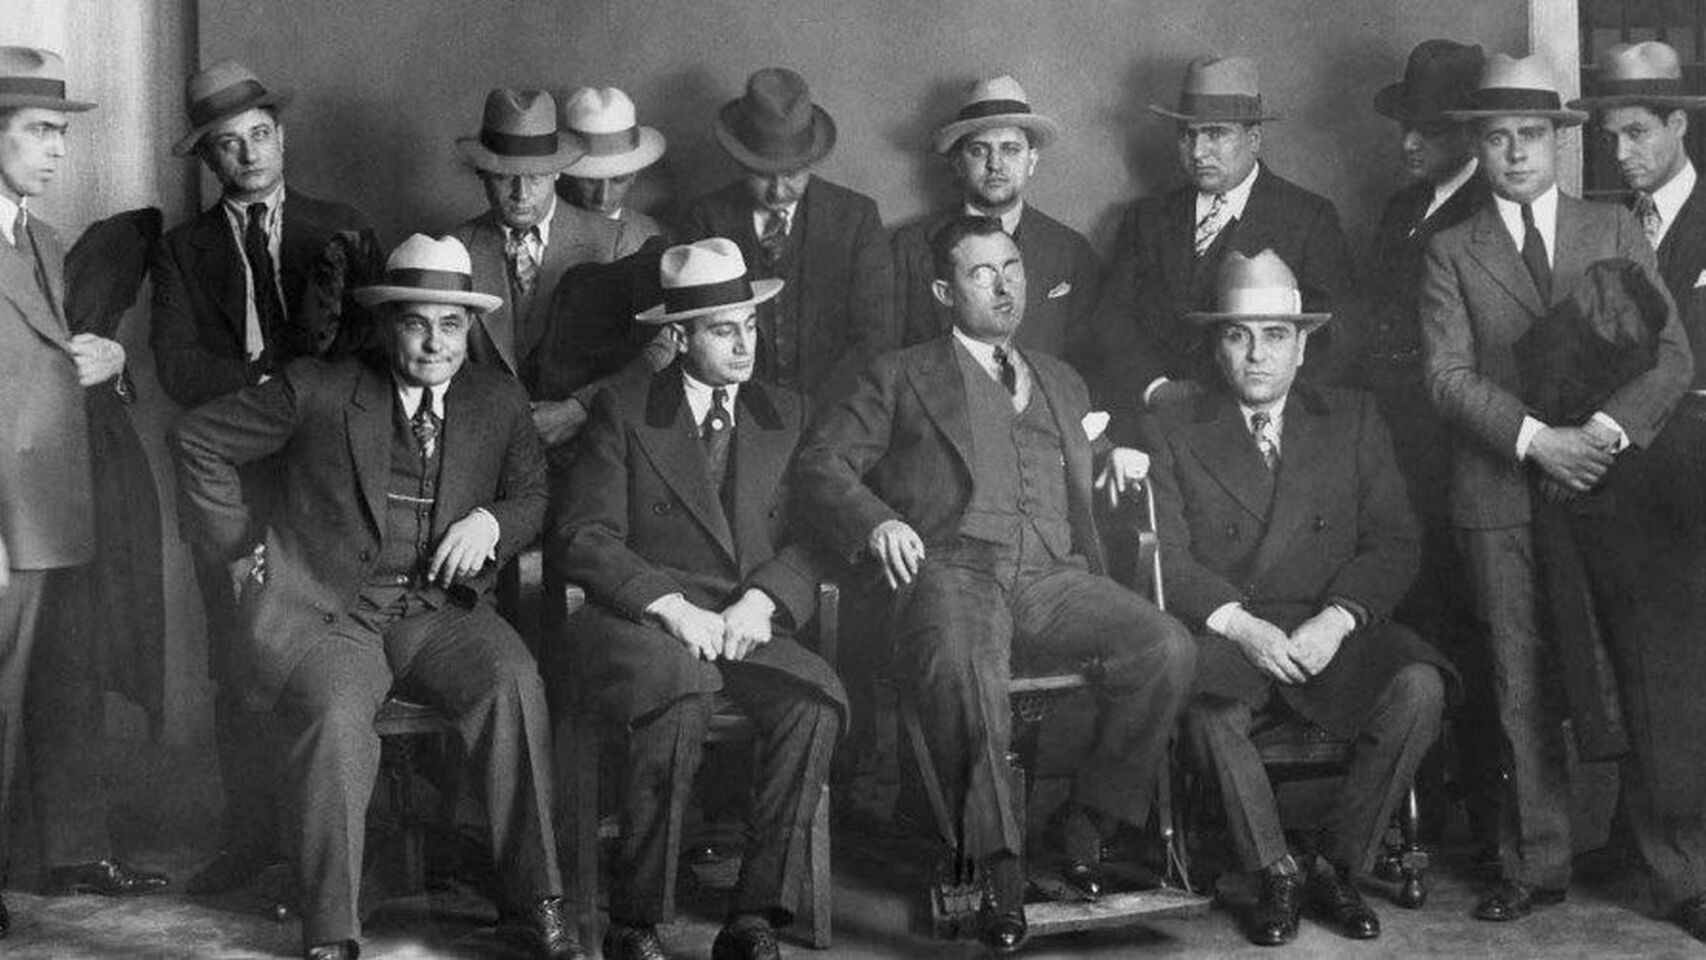
\includegraphics[width = 0.8\textwidth]{img/cosa_nostra}

{\small Cosa Nostra's `The Commission'}

\vspace{20pt}

\begin{itemize}
  \item How does a state resembles a criminal organization?
\end{itemize}

\end{frame}

% \begin{frame}
% \frametitle{The state as a criminal organization}
% \centering
%
% \begin{itemize}
%   \item Protection racket: offering protection (services) in exchange for taxes
%   \item Only works if there's territorial monopoly
%   \item Use of violence as an enforcing mechanism
% \end{itemize}
%
% \end{frame}

\begin{frame}
\frametitle{The state as a criminal organization}
\centering

\begin{minipage}{0.63\textwidth}\centering
\begin{itemize}
\item \textit{Pizzo} in Italy (Mafia in Sicily, 'Ndrangheta in Calabria, Camorra in Campania, etc)
\item Protection money paid by local businesses to a criminal organization
\item If you pay you get access to services: protection, speedy bureaucracy, resolution of conflicts...
\item If you don't pay? Business destroyed
\item Who do you pay? Local organization
\end{itemize}
\end{minipage}\hfill
\begin{minipage}{0.36\textwidth}\centering
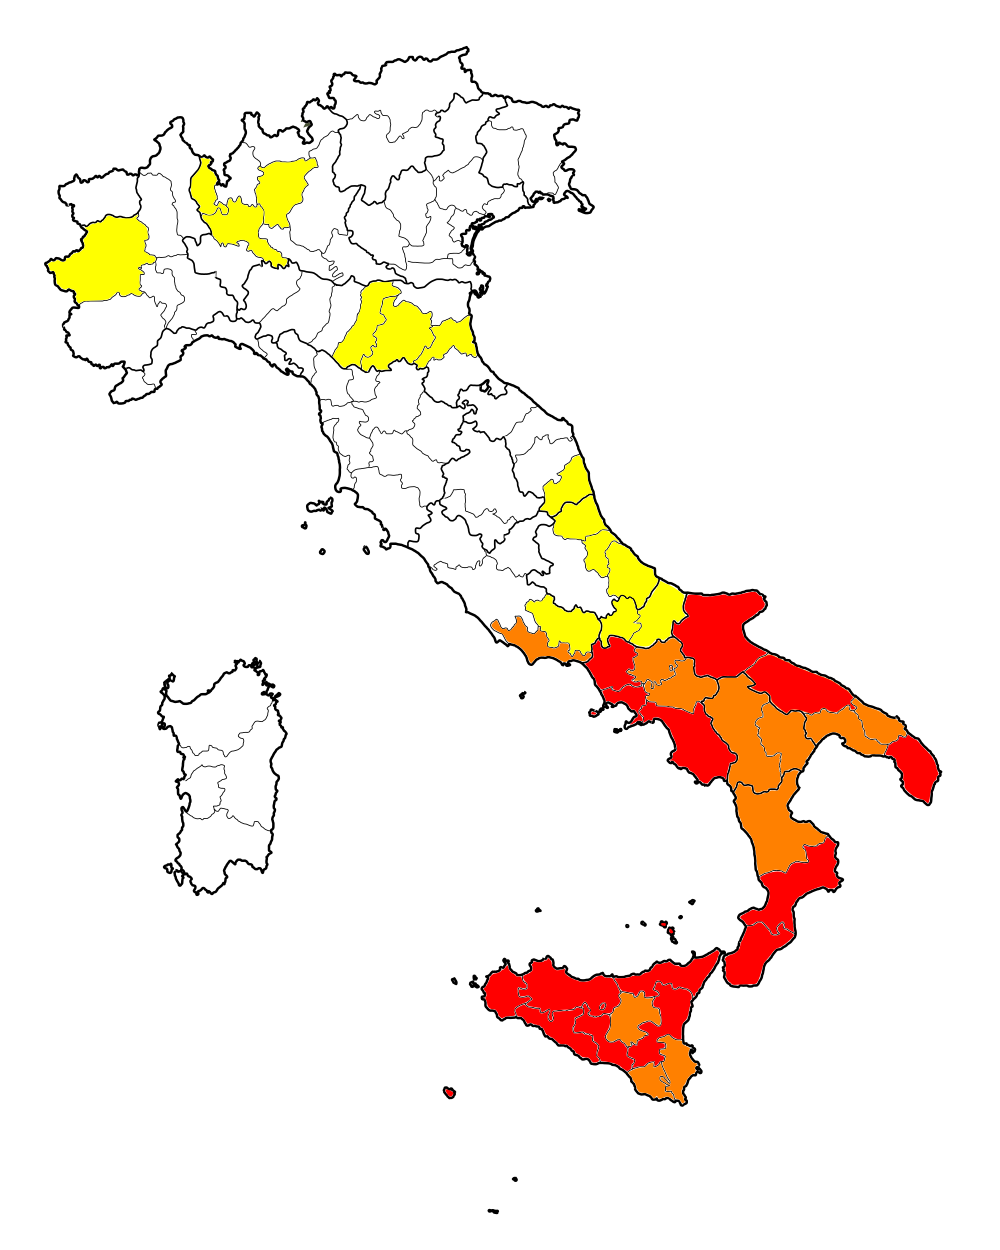
\includegraphics[width = 0.9\textwidth]{img/italy_pizzo}\\
{\small Extortion in Italy, 2008}\\\vspace{5pt}
{\tiny Source: Daygum (Wikipedia),\\data from Confesercenti Survey\\}
\end{minipage}

\end{frame}

\begin{frame}
\frametitle{The state as a criminal organization}
\centering

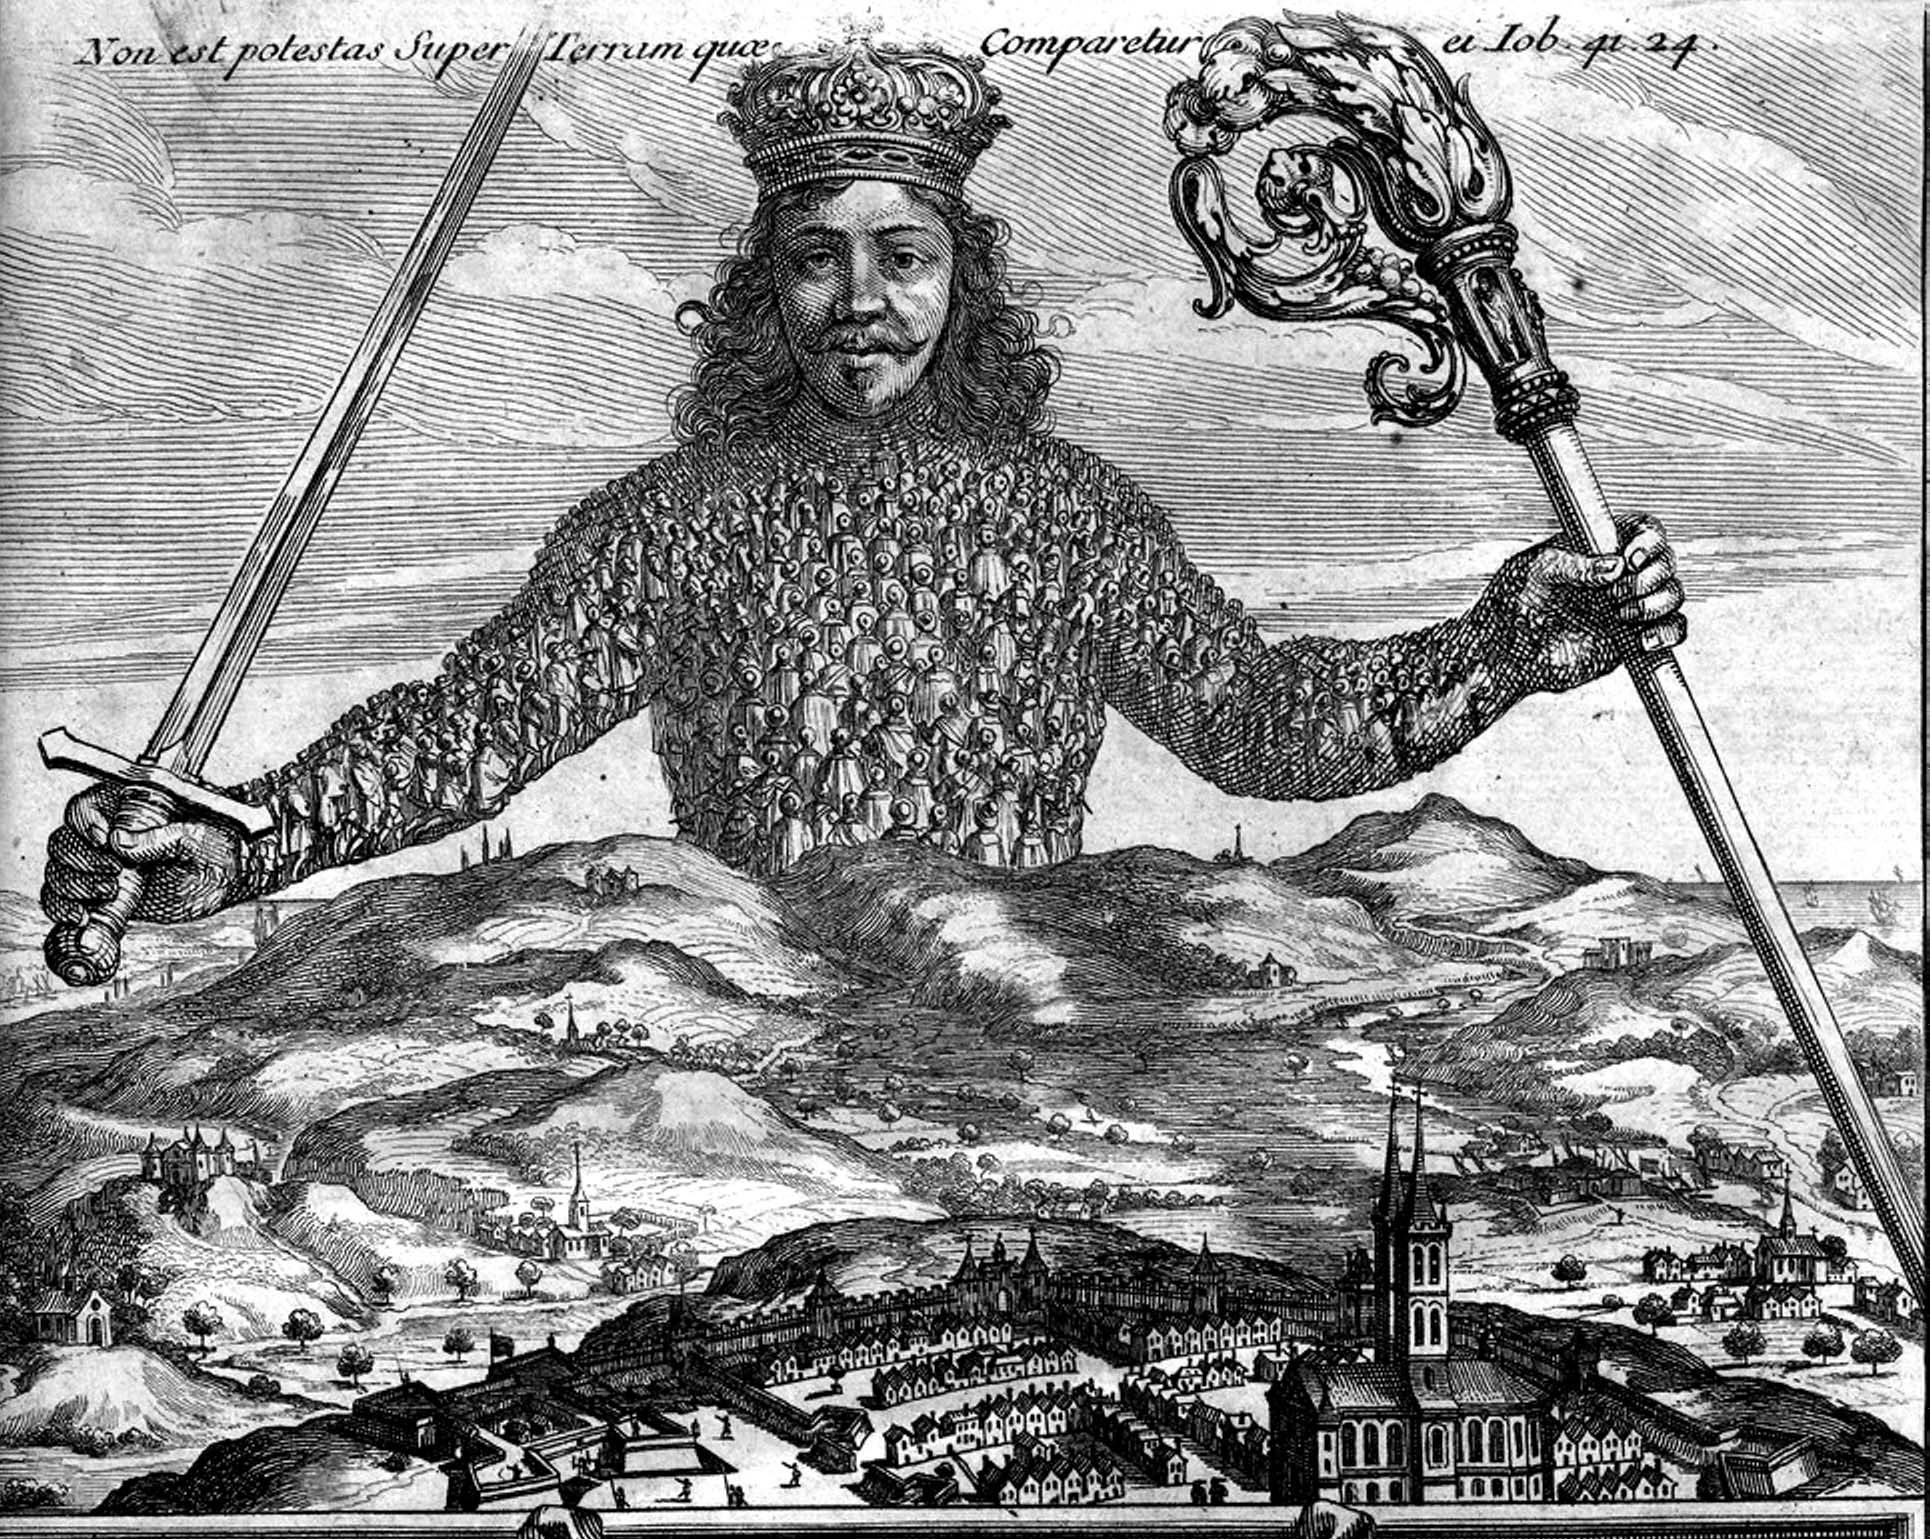
\includegraphics[width = 0.7\textwidth]{img/leviathan}

\vspace{20pt}

{\small Hobbes' \textit{Leviathan}}

\end{frame}


% ----------------------------------------------------
\begin{frame}
\frametitle{The origins of states}
\centering

\begin{itemize}
  \item How did the modern state emerge?
\end{itemize}

\end{frame}
% ----------------------------------------------------

\begin{frame}
\frametitle{Charles Tilly and the origins of European states}
\centering

\begin{minipage}{0.66\textwidth}\centering
\begin{itemize}
\item State-formation process in Europe
\item The protection racket idea: kings and rulers were not different from the initial competitors (legitimacy happens afterwards)
\item Dual process of establishing a monopoly of violence and building state institutions
% \item<2-> \textbf{``War made the state and the state made war''}
\end{itemize}
\end{minipage}\hfill
\begin{minipage}{0.33\textwidth}\centering
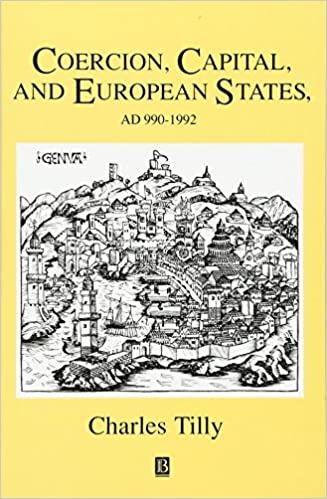
\includegraphics[width = 0.9\textwidth]{img/tilly_book}\\\vspace{5pt}
{\small Charles Tilly (1990)}
\end{minipage}

\end{frame}

\begin{frame}
\frametitle{War-making and state-making in Europe}
\centering

\begin{minipage}{0.49\textwidth}\centering
  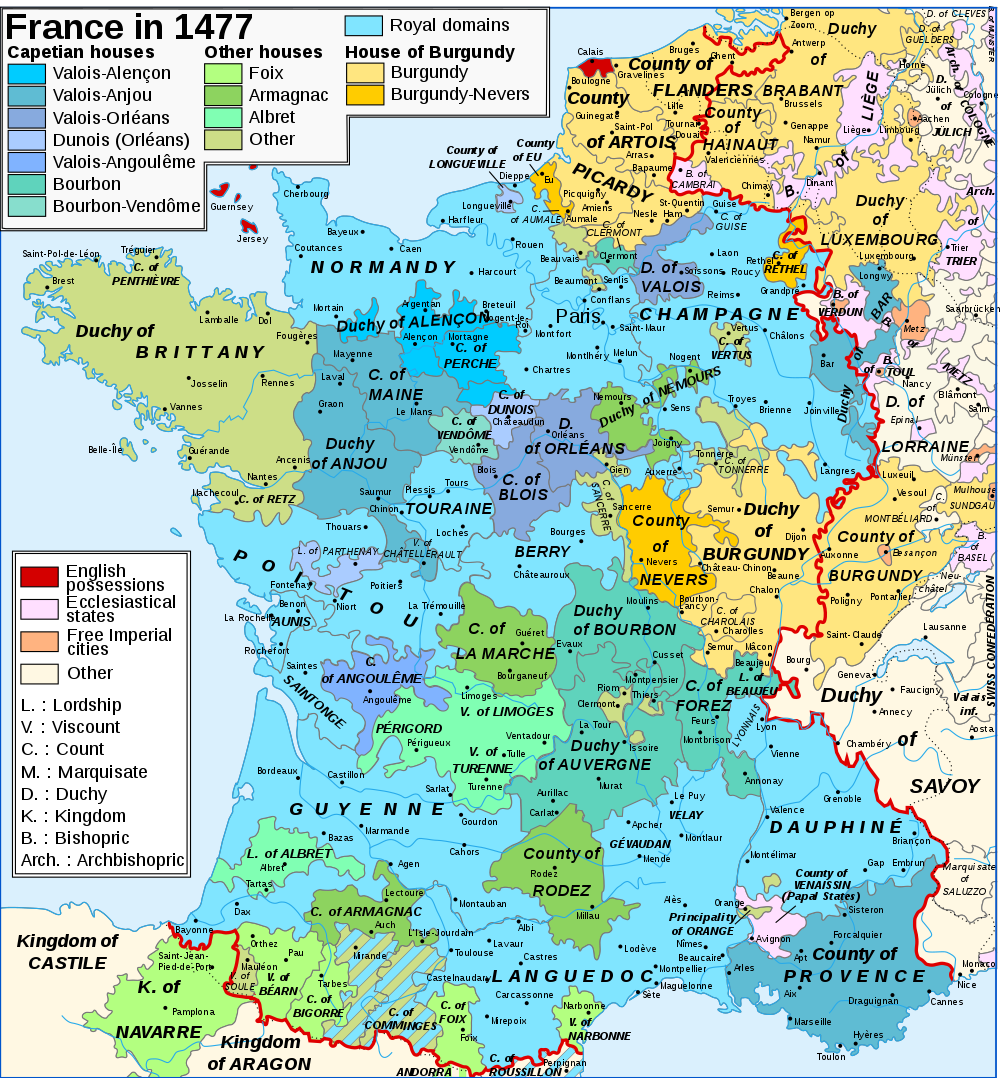
\includegraphics[width = \textwidth]{img/france1477}\\
  {\small France around 1477}
\end{minipage}\hfill
\begin{minipage}{0.49\textwidth}\centering
  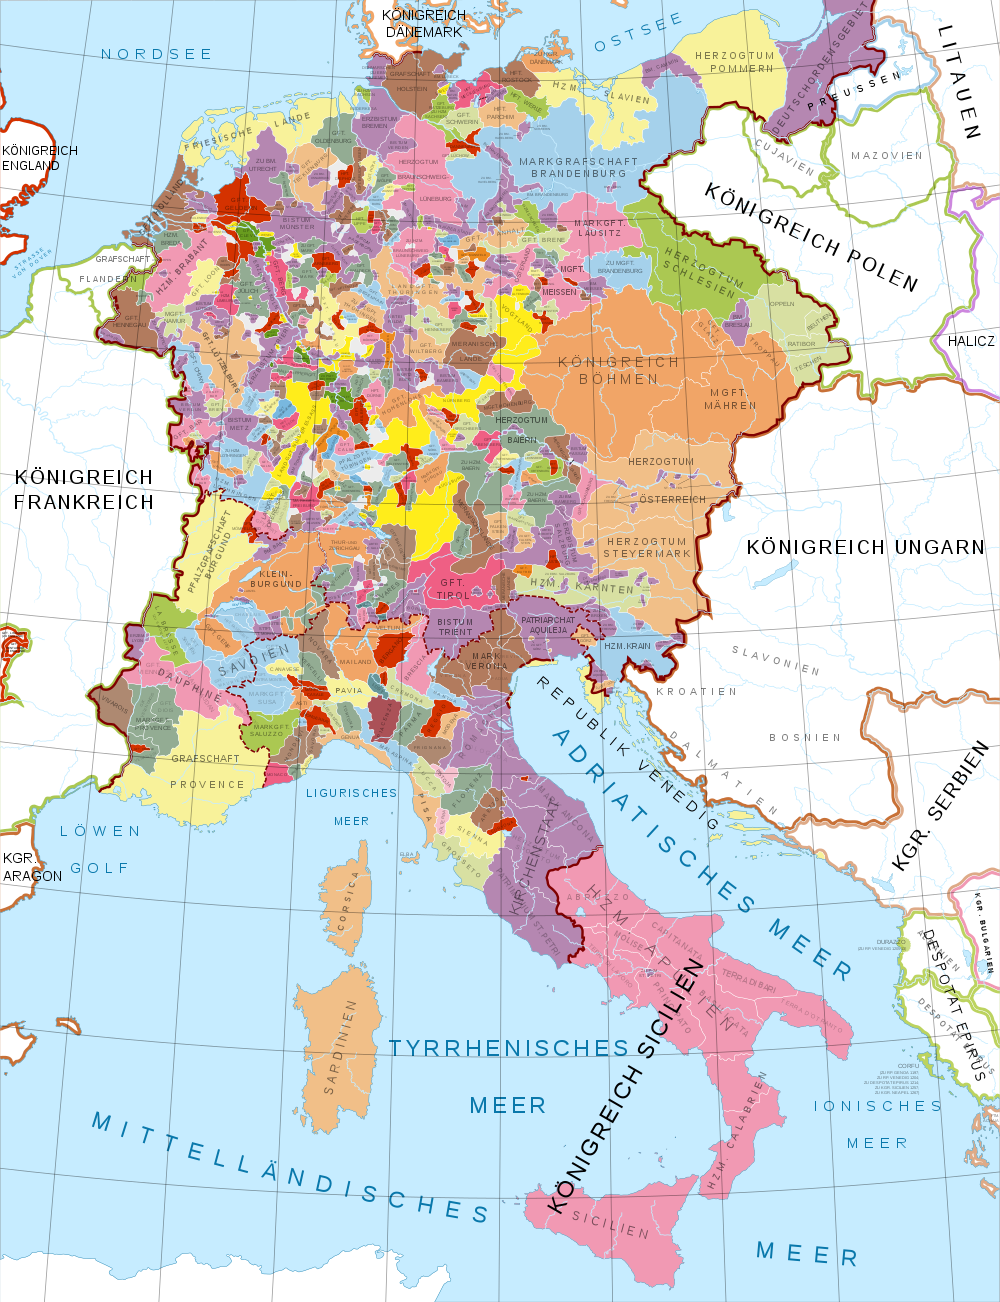
\includegraphics[width = \textwidth]{img/holy_roman_empire_1200}\\
  {\small Holy Roman Empire around 1200}
\end{minipage}

\end{frame}

\begin{frame}
\frametitle{War-making}
\centering

\begin{itemize}
\item Early states in Europe competed for territory and power
\item Context of Feudalism:
  \begin{itemize}
    \item Decentralized means of violence, fragmented rule
    \item Pressures for war-making: conquer or be conquered
  \end{itemize}
\item Kings or powerful lords did not use \textit{direct rule}, but relied on intermediaries
\begin{itemize}
  \item Direct vs indirect rule
\end{itemize}
\item<2-> \BGyellow{Innovations in the technology of war} changed it all: war became more and more expensive
\end{itemize}

\end{frame}

\begin{frame}
\frametitle{State-making}
\centering

\begin{itemize}
\item In the process of waging war against external enemies, two more things happened
\item[1.] \BGyellow{Bureaucracy}
  \begin{itemize}
    \item How do you finance the war? Taxing the population
    \item Tax and administration institutions developed
  \end{itemize}
\item<2->[2.] \BGyellow{Internal monopoly}
\begin{itemize}
  \item The intermediaries in \textit{indirect rule} (feudal lords, etc) were also potential enemies to the king
  \item Gaining power among internal threats, establishing monopoly of violence (not always successfully)
\end{itemize}
\item<3-> Later on: censuses, modern bureaucracy, police
\end{itemize}

\end{frame}

\begin{frame}
\frametitle{War-making and state-making}
\centering

\begin{itemize}
\item \BGyellow{``War made the state and the state made war''}
\item[]
\item<2-> Different from other conceptions of the origins of the state
\begin{itemize}
  \item e.g. social contract
\end{itemize}
\item<2-> Rooted in security concerns: remember that protection threats (esp. external) is usually the idea of a minimum state
\begin{itemize}
  \item ``Love-hate relationship between state makers and pirates or bandits''
\end{itemize}
\item<2-> The service side of the state was developed as a response to population resistance to coercive governance
\end{itemize}

\end{frame}


\begin{frame}
\frametitle{War and the state development process}
\centering

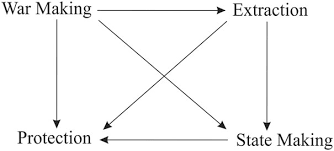
\includegraphics[width = 0.5\textwidth]{img/tilly_causal_chain}

\vspace{20pt}

{\small Tilly's causal chain of European state-making}

\vspace{20pt}

\begin{itemize}
  \item It all starts with war-making: states are a by-product of rulers' efforts to increase the means of war
  \item And it's all about violence: coercive violence is used to develop the monopoly of legitimate violence
\end{itemize}

\end{frame}

\begin{frame}
\frametitle{War-making and state-making}
\centering

\begin{quote}
  By the later eighteenth century, through most of Europe, monarchs controlled permanent, military forces that rivaled those of their neighbors and far exceeded any other organized armed force within their own territories. The state's monopoly of large-scale violence was turning from theory to practice. (Tilly 1985, p. 174)
\end{quote}

\begin{itemize}
\item Westphalian international system ``fully developed''
\item<2-> Shift to (more costly) direct rule after French Revolution
\item<2-> Only possible after kings won previous ``civil wars''
  \begin{itemize}
    \item The development of the police in the 19th century was the latest step, reaching out the most local challengers
  \end{itemize}
% \item State-making $\neq$ peace-making
\end{itemize}

\end{frame}

% THE TWO IMPLICATIONS
% -- Popular resistance mattered, because the higher it was, the more concessions state makers had to do (with its later path-dep implications)
% -- The relative balance of the four activities defined the future state


\begin{frame}
\frametitle{Bringing the international system in}
\centering

\begin{itemize}
  \item Early on, no distinction between internal and external threats
  \item Later on, war as major moving force of the international system, with similar dynamics as in internal state making (violence)
  \item Peace of Westphalia in 1648: clear borders of sovereignty emerge and after each war, states are re-defined (usually decreasing in number)
  \begin{itemize}
    \item if you think about this, how to make sense of `pre-Westphalian' civil wars?
  \end{itemize}
\end{itemize}

\end{frame}

% \begin{frame}
% \frametitle{War and state services in the XXth century?}
% \centering
%
% \begin{minipage}{0.66\textwidth}\centering
% \begin{itemize}
%   \item The selection process among states because of warfare does not work anymore
%   \item But maybe the logic of offering something in exchange for contributing to the efforts of war does
%   \item World War II and mass mobilization led to an increase in tax to the wealthy as compensation
% \end{itemize}
% \end{minipage}\hfill
% \begin{minipage}{0.33\textwidth}\centering
% \includegraphics[width = 0.9\textwidth]{img/scheve-stasavage}\\
% {\small Kenneth Scheve \& David Stasavage (2016)}
% \end{minipage}
%
% \end{frame}

% \begin{frame}
% \frametitle{Can we generalize from European history?}
% \centering
%
% \begin{itemize}
%   \item Tilly's bellicist theory left one question open:
%   \item[] ``The fact that European states formed in a certain way, then imposed their power on the rest of the world, guarantees that non-European experience will be different''
%   \item So how or why did it happen outside of Europe?
%   \item Also related to the other part of the theory: capital development
% \end{itemize}
%
% \end{frame}

\begin{frame}
\frametitle{Can we generalize from European history?}
\centering

\begin{minipage}{0.6\textwidth}\centering
  \begin{itemize}
    \item<2-> Absence of international wars in \BGyellow{Africa} explains weak states
    \begin{itemize}
      \item Historically low population density, rough terrain: no state emergence
      \item ``Addis rule'' froze borders after decolonization
    \end{itemize}
    \item<3-> Problem: there are some disputes and also these states face much more internal than external threats, shouldn't this be an incentive for state-building or work the same way?
  \end{itemize}
\end{minipage}\hfill
\begin{minipage}{0.4\textwidth}\centering
  \only<2->{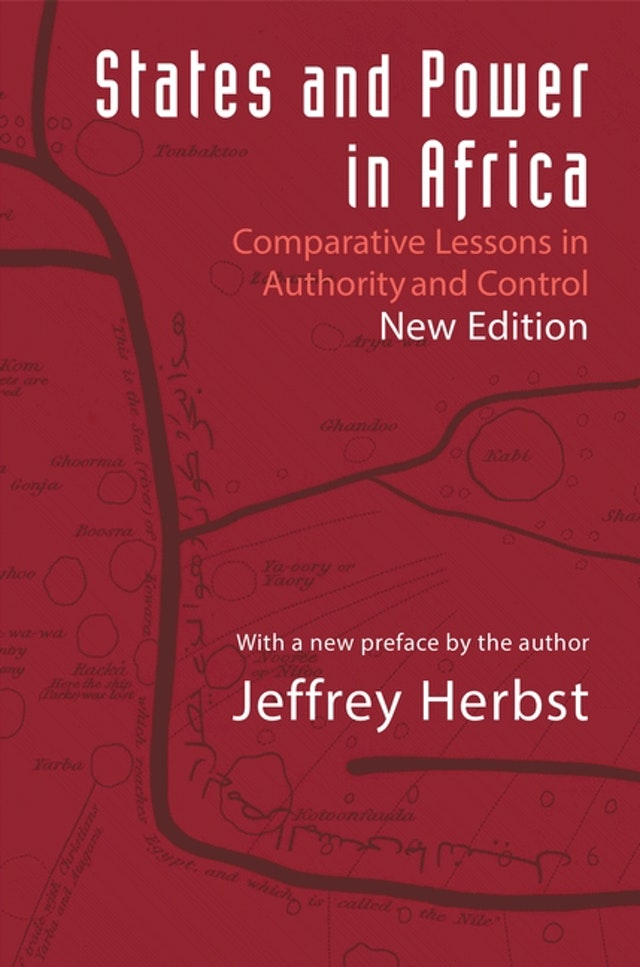
\includegraphics[width = 0.8\textwidth]{img/herbst}\\
  {\small Jeffrey Herbst (2015)}}
\end{minipage}

\end{frame}

\begin{frame}
\frametitle{Can we generalize from European history?}
\centering

\begin{itemize}[<+->]
  \item Tribute-taking empires in \BGyellow{Asia} (Victoria Hui, \textit{War and State Formation in Ancient China and Early Modern Europe})
  \item Existence of capital in \BGyellow{Latin America} (Miguel A Centeno, \textit{Blood and debt: War and the nation-state in Latin America})
  \item[]
  \item One pressing question today is: \textbf{How should we see internal conflicts? Do they strengthen of weaker state-formation?}
\end{itemize}

\end{frame}


% ----------------------------------------------------
\begin{frame}
\frametitle{Can we generalize from European history?}
\centering

\begin{minipage}{0.6\textwidth}\centering
  \begin{itemize}
    \only<1>{\item Some have tried to actually generalize, and understand why and how it was different in Europe}
  \end{itemize}
\end{minipage}\hfill
\begin{minipage}{0.4\textwidth}\centering
  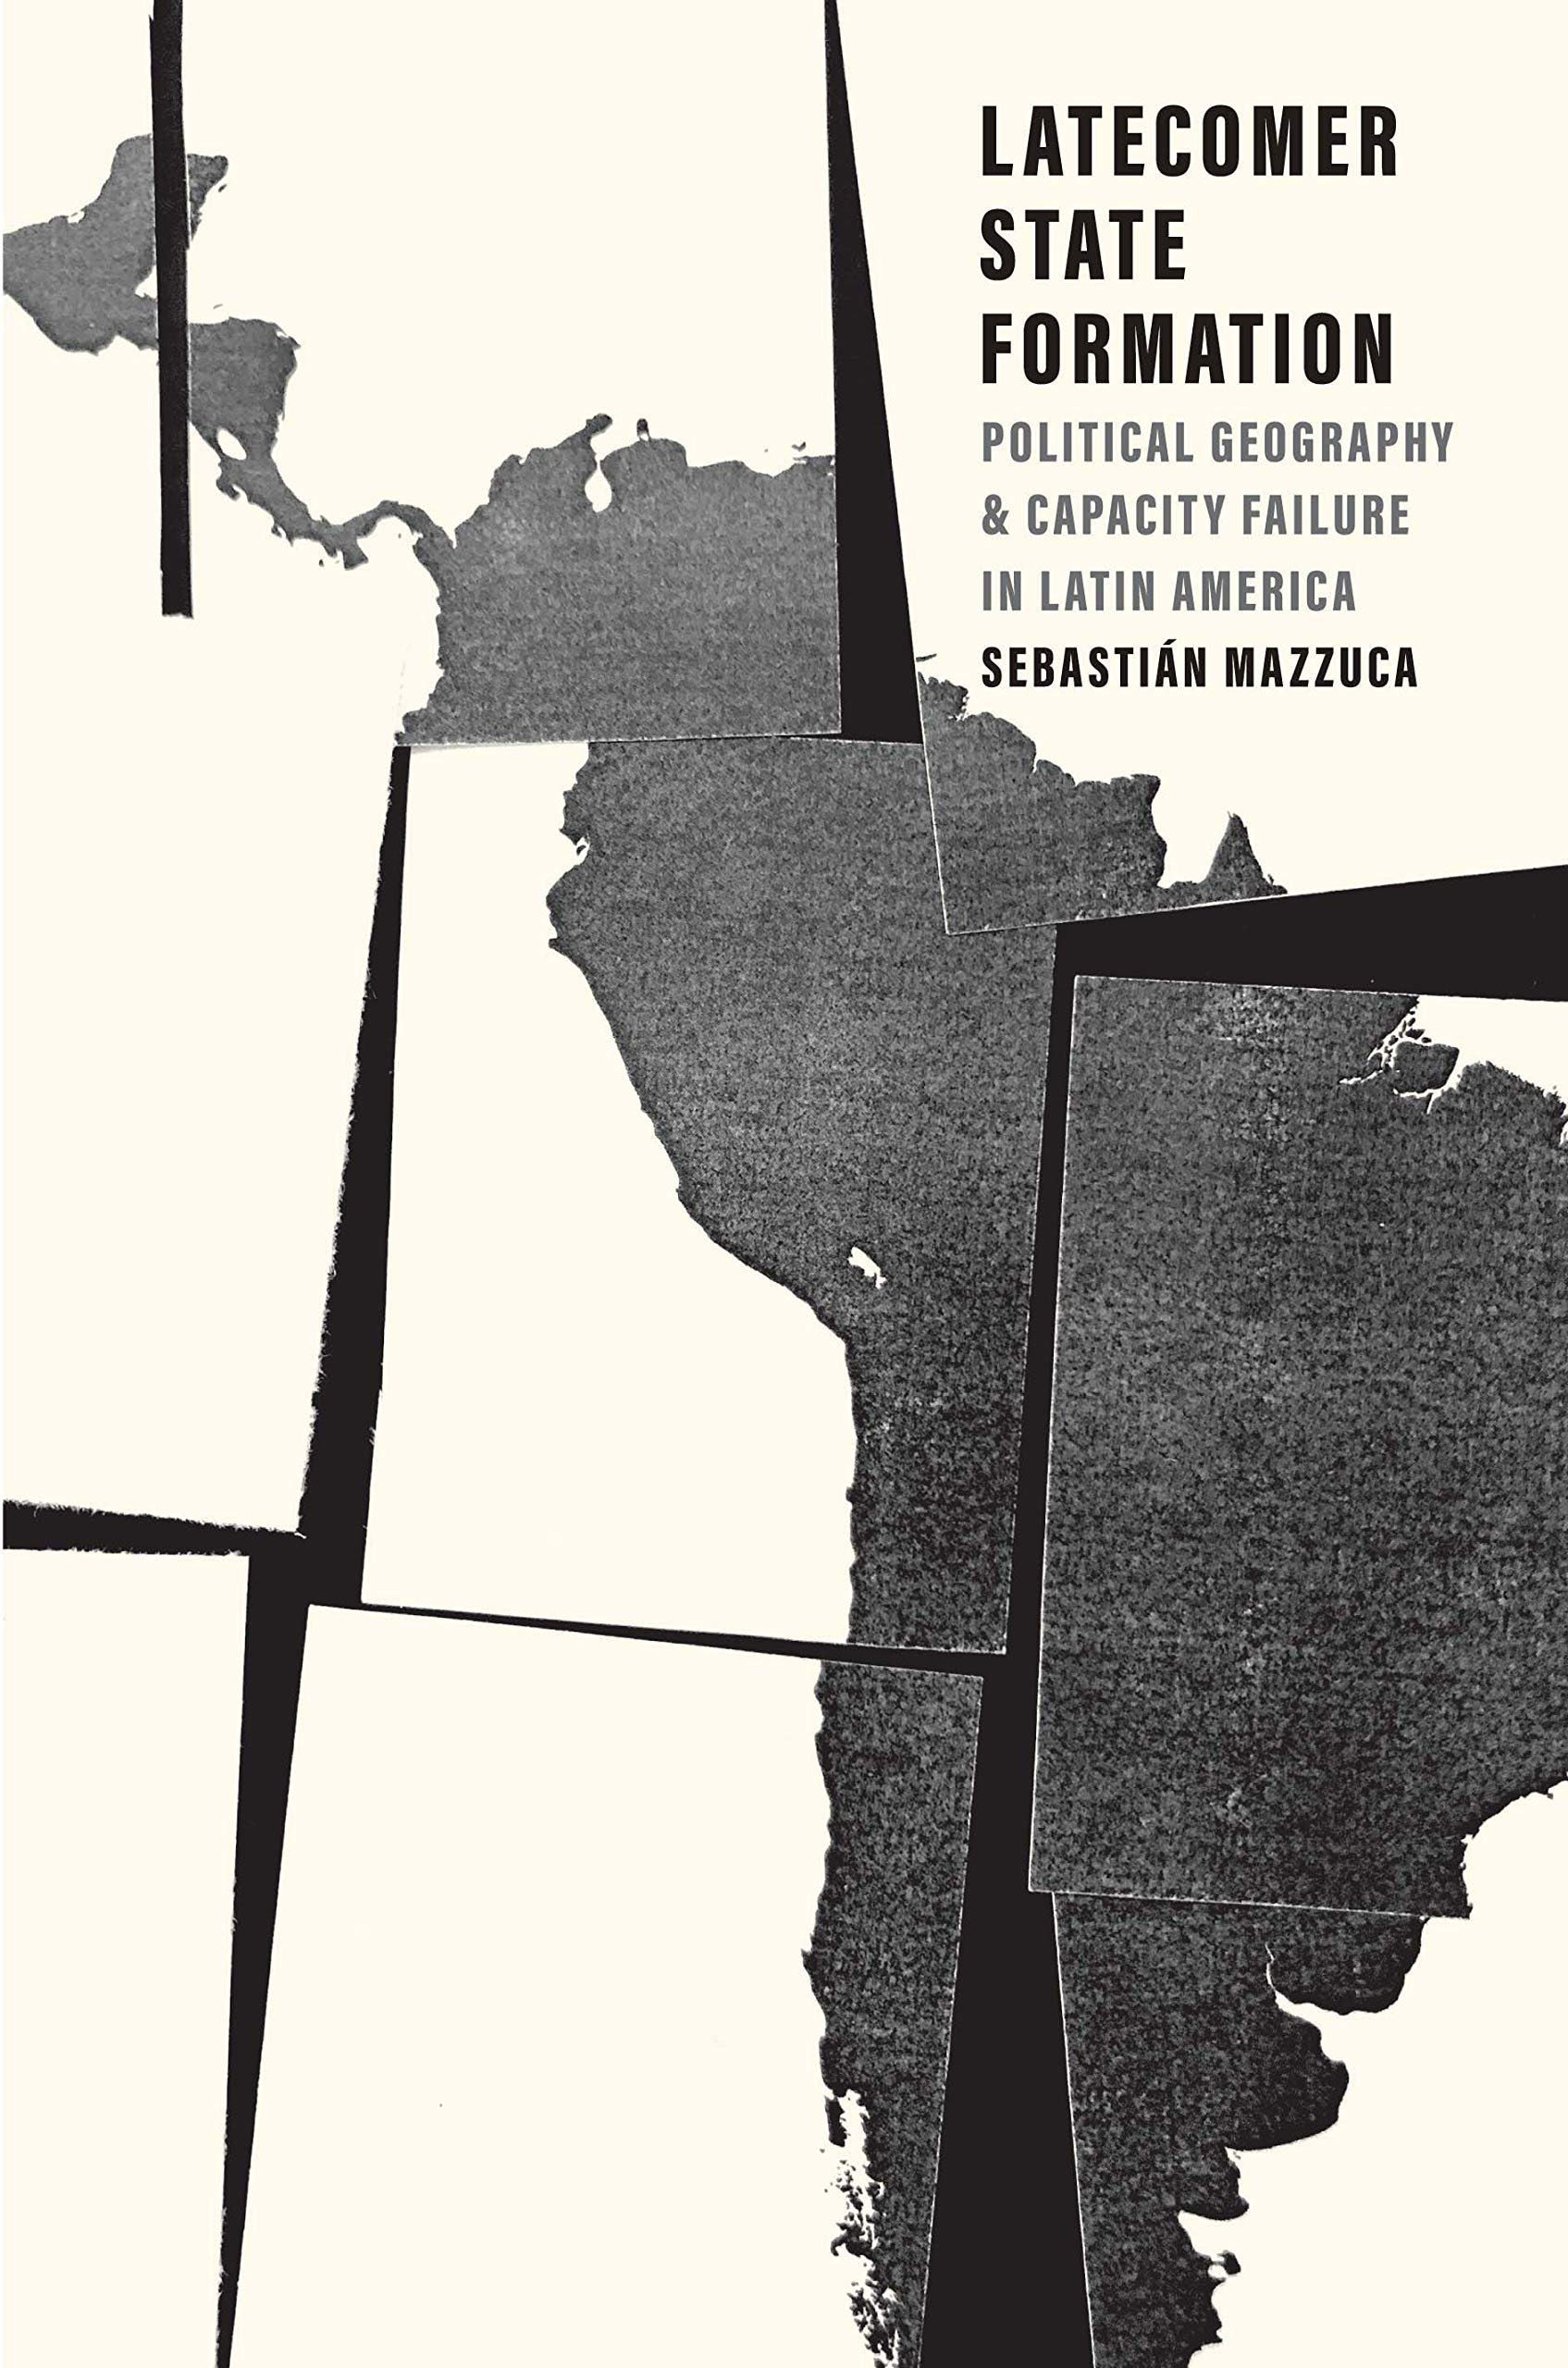
\includegraphics[width = 0.8\textwidth]{img/mazzuca_book}\\
  {\small Mazzuca (2021)}
\end{minipage}

\end{frame}
% ----------------------------------------------------

% ----------------------------------------------------
\begin{frame}
\frametitle{Can we generalize from European history?}
\centering

\begin{minipage}{0.6\textwidth}\centering
  \begin{itemize}
    \only<1>{\item Some have tried to actually generalize, and understand why and how it was different in Europe}
    \item<2-> \BGyellow{State formation} (monopoly of violence within delimited borders) vs \BGyellow{state building} (switch from patrimonial to bureaucratic administration)
    \begin{itemize}
      \item They can happen at the same time (Europe), or not
    \end{itemize}
    \item<3-> State formation in LatAm took place when capitalism, rather than war, ruled internationally
    \item<3-> Because of pursuing benefits of trade, LA countries created weak states, with patrimonial structures, etc
  \end{itemize}
\end{minipage}\hfill
\begin{minipage}{0.4\textwidth}\centering
  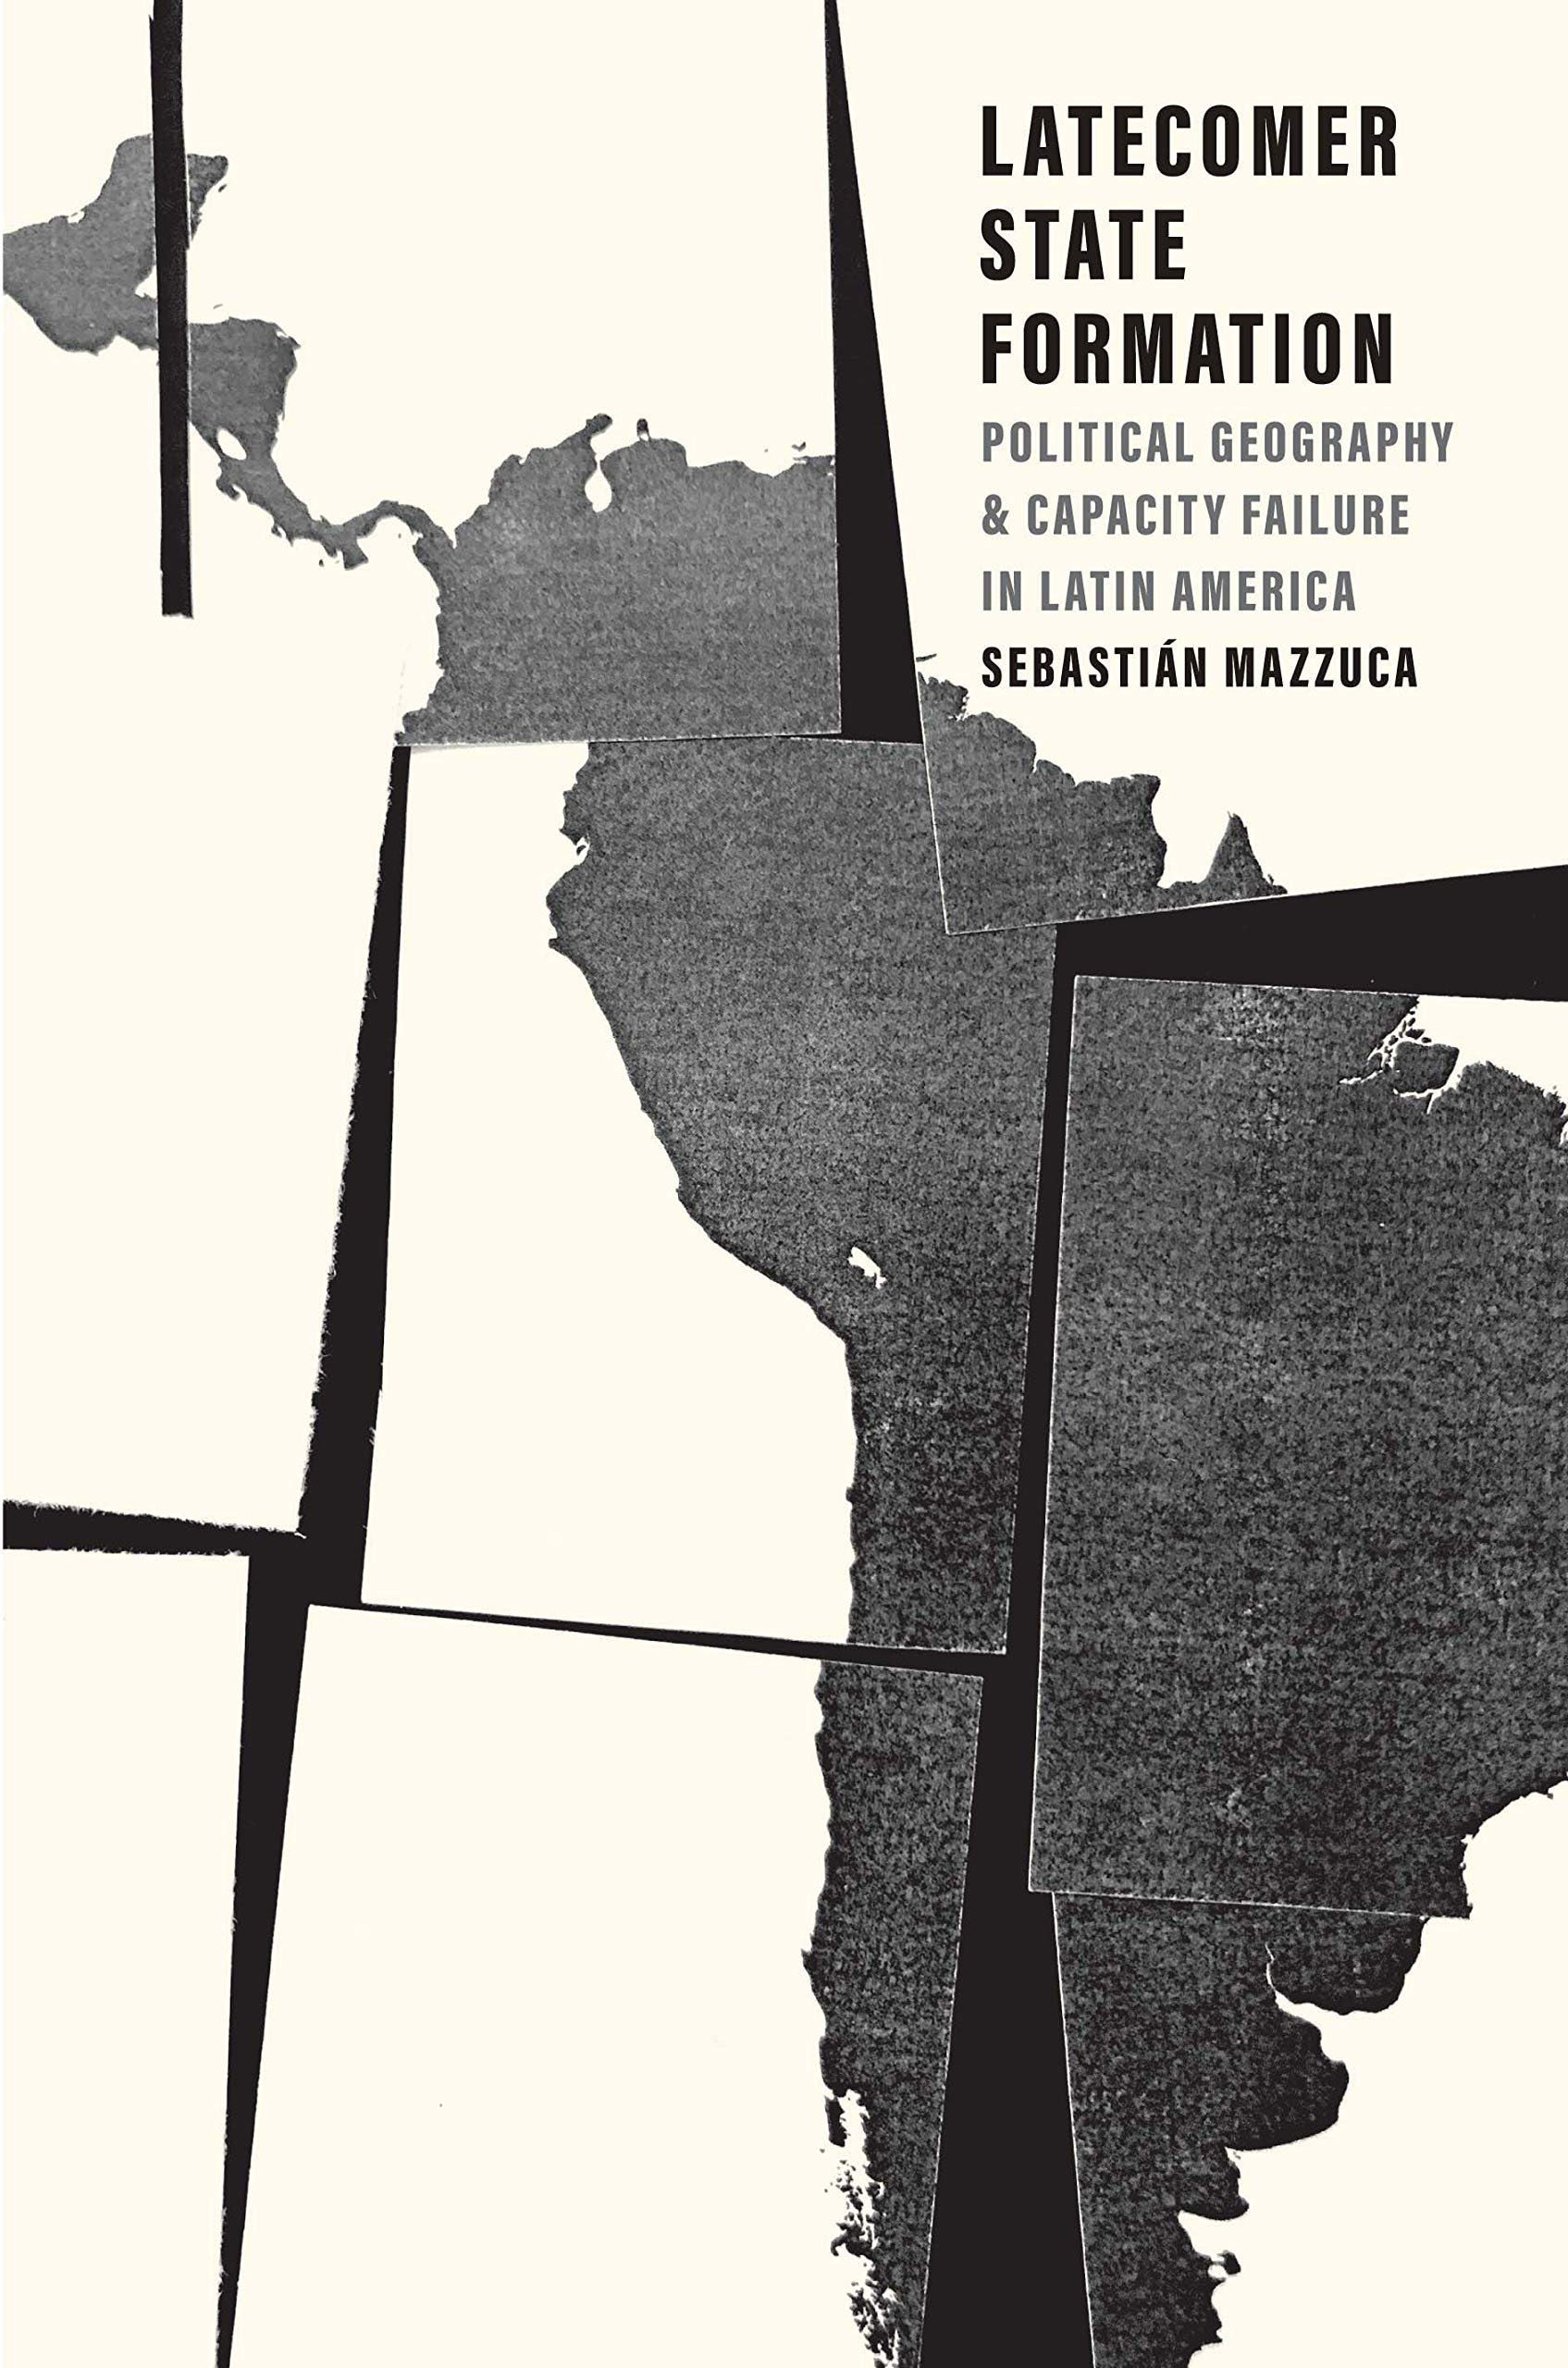
\includegraphics[width = 0.8\textwidth]{img/mazzuca_book}\\
  {\small Mazzuca (2021)}
\end{minipage}

\end{frame}
% ----------------------------------------------------

% % ----------------------------------------------------
% \begin{frame}
% \frametitle{Generalizing from European history}
% \centering
%
% 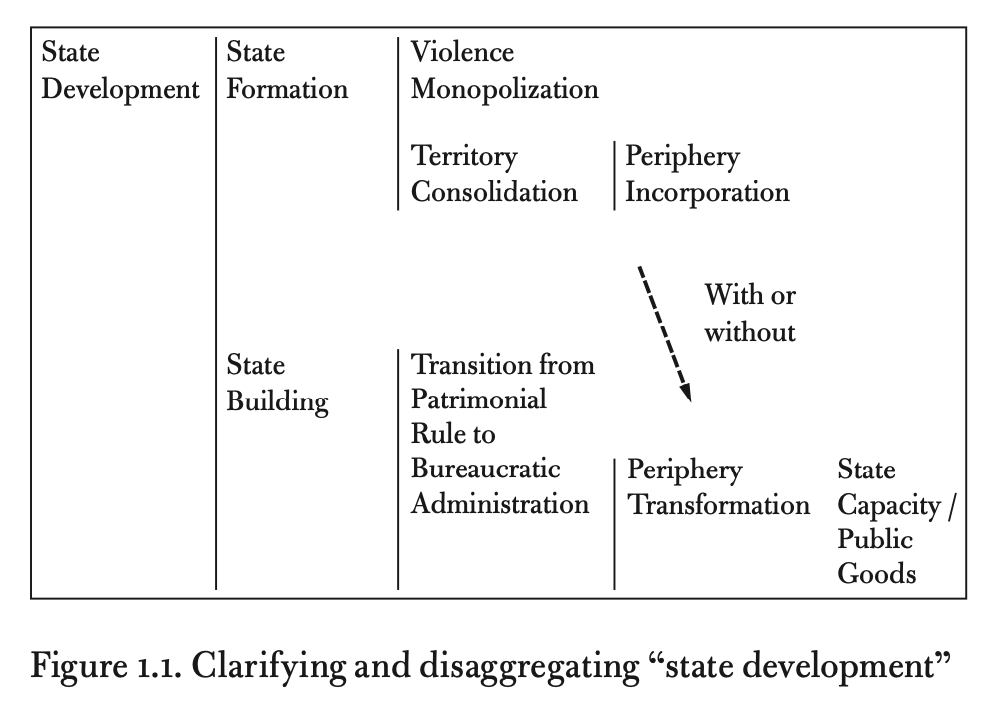
\includegraphics[width = 0.75\textwidth]{img/mazzuca_table1}
%
% \end{frame}
% % ----------------------------------------------------

% ----------------------------------------------------
\begin{frame}
\frametitle{Generalizing from European history}
\centering

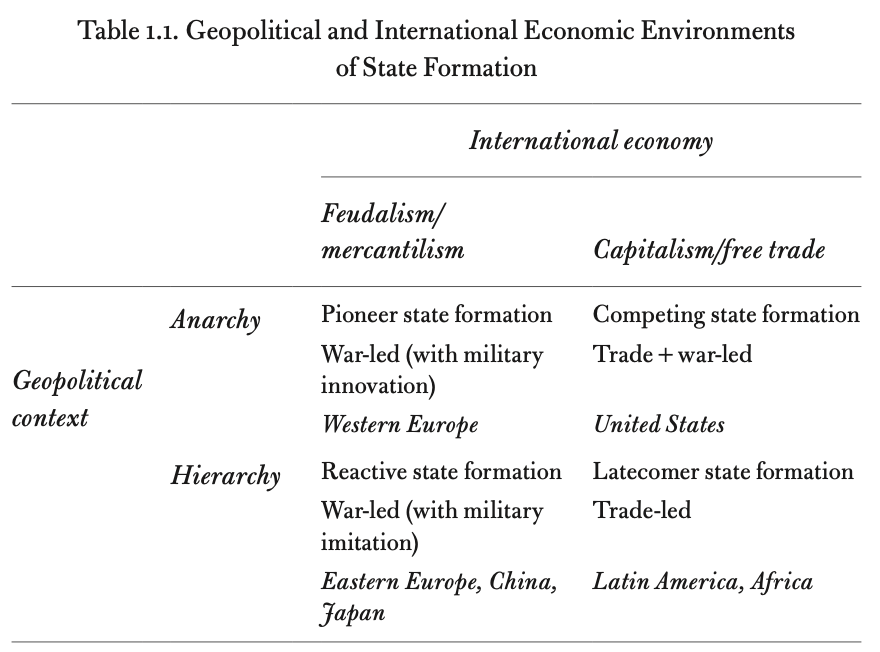
\includegraphics[width = 0.85\textwidth]{img/mazzuca_table2}

\end{frame}
% ----------------------------------------------------


\begin{frame}
\frametitle{Two critiques to the bellicist theory}
\centering

\begin{itemize}
  \only<1>{\item[1.] \textbf{European system environment is} \BGyellow{\textbf{not exogenous}}}
  \only<1>{\item Why were so many independent states in Europe fighting each other?}
  \only<1>{\item Not random, it needs to be explained, maybe it has to do with the failure of other systems}
  \only<2>{\item[2.] \textbf{Which \BGyellow{micro-level mechanisms} explain that war-making increases state capacity?}}
  \only<2>{\item States can increase internal capacity, but can also look for allies, bandwagon on stronger powers, etc}
  \only<2>{\item In other words, it does \textit{not} always happens this way, fighting could also lead to   chaos and state collapse, and external threats do not necessarily lead to stronger states}
  \item[]
  \item[] {\small \textit{See}: Hendrik Spruyt in \textit{Does War Make States?} (CUP, 2017)}
\end{itemize}

\end{frame}

\begin{frame}
\frametitle{The role of legitimacy}
\centering

\begin{itemize}
  \item So are states really like criminal protection rackets? Bellicist theory assumes that at the beginning there were many competing authorities offering protection and kings were just the better providers
  \item But \BGyellow{legitimacy could have played a role}: maybe people did care about who ended up ruling over all
  \item Kings were not exactly the same as minor lords: they could claim legitimacy and loyalty, and emerge as the ultimate defenders
  \item Think of situations of fragmented rule without cultural unity: e.g. warlords in Somalia
  \begin{itemize}
    \item (though we cannot talk about nationalism in Early Modern Europe)
  \end{itemize}
\end{itemize}

% check last paragraph of Tilly 1985!
\end{frame}

\begin{frame}
\frametitle{What is this all about}
\centering

\begin{itemize}
  \item War and violence and the state are deeply related from the start
  \item Coercion and the monopoly of violence still define many if not all problems of political order today
  \item<2-> Very relevant questions for contexts of civil wars or state collapse
  \begin{itemize}
    \item Somalia, DRC, etc
  \end{itemize}
  \item<2-> Do preferences for centralized or decentralized force matter?
  \begin{itemize}[<+->]
    \item War and state formation in multi-ethnic countries?
    \item Why Mafia flourished in southern Italy? And why do we see higher mobilization against it today? (\textit{Addiopizzo} movement)
  \end{itemize}
\end{itemize}

\end{frame}


\begin{frame}
\frametitle{Extra: Empirical evidence}
\centering

\begin{minipage}{0.65\textwidth}\centering
  \begin{itemize}
    \item States created statistics, so it's difficult to study its formation empirically
    % \item Sánchez de la Sierra (2020) ``On the Origins of the State: Stationary Bandits and Taxation in Eastern Congo'' (\textit{Journal of Political Economy})
    \item Q: When do \BGyellow{`stationary bandits'} emerge?
    \item<2-> Studying `roving bands` in DRC, and analyzing price of coltan and gold
    \begin{itemize}
      \item coltan is bulky, but not gold
    \end{itemize}
    \item<3-> When coltan price goes up, rebels establish monopoly of violence in mines
    \item<3-> When gold price goes up, rebels tax villages and provide services
    \begin{itemize}
      \item i.e. expropriation $\rightarrow$ state
    \end{itemize}
  \end{itemize}
\end{minipage}\hfill
\begin{minipage}{0.34\textwidth}\centering
  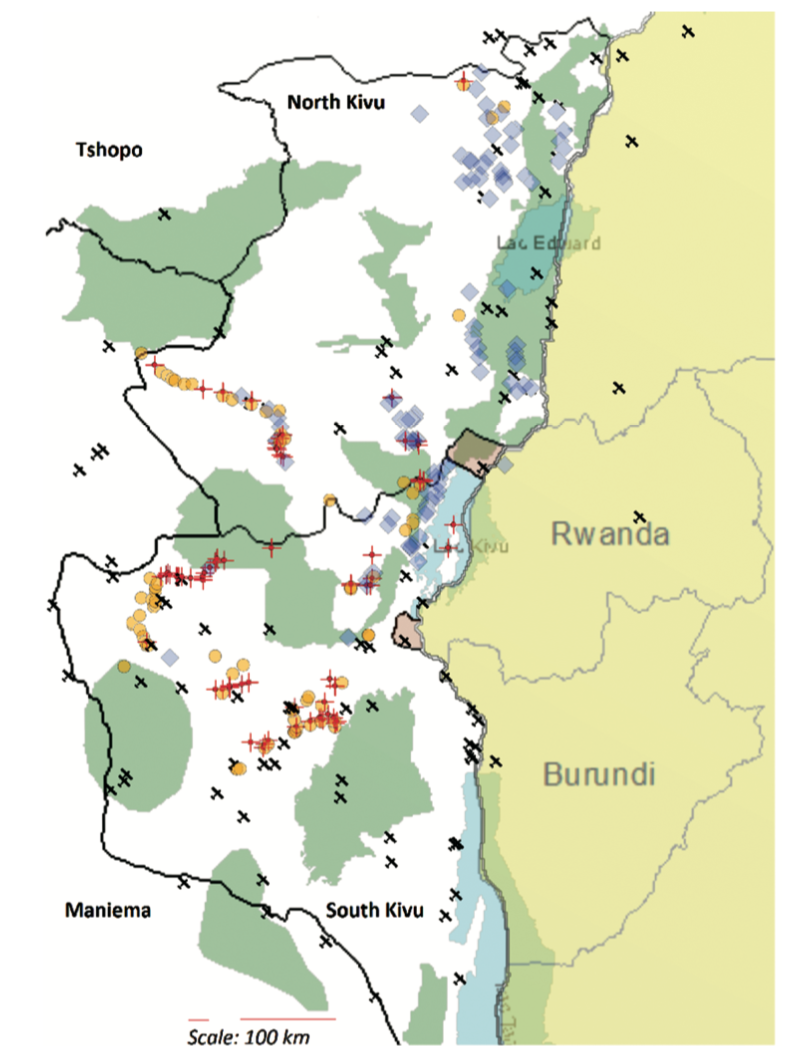
\includegraphics[width = \textwidth]{img/sanchez_de_la_sierra_sample}\\
  {\footnotesize Sánchez de la Sierra (2020)\\\textit{Journal of Political Economy}\\}
\end{minipage}

\end{frame}

\begin{frame}
\frametitle{Extra: James C. Scott on the origin of state}
\centering

\begin{minipage}{0.6\textwidth}\centering
  \begin{itemize}
    \item Against the usual idea that people freely chose to settle and form states
    \item The origin of the state matched with violent coercion, diseases, and slavery
    \item States `domesticated' humans as much as they domesticated animals
  \end{itemize}
\end{minipage}\hfill
\begin{minipage}{0.39\textwidth}\centering
  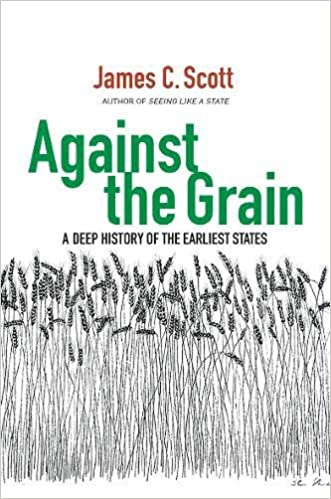
\includegraphics[width = 0.9\textwidth]{img/scott_against}\\
  James C. Scott (2017)
\end{minipage}

\end{frame}

% % ----------------------------------------------------
% \begin{frame}
% \frametitle{What about actual gangs?}
% \centering
%
% 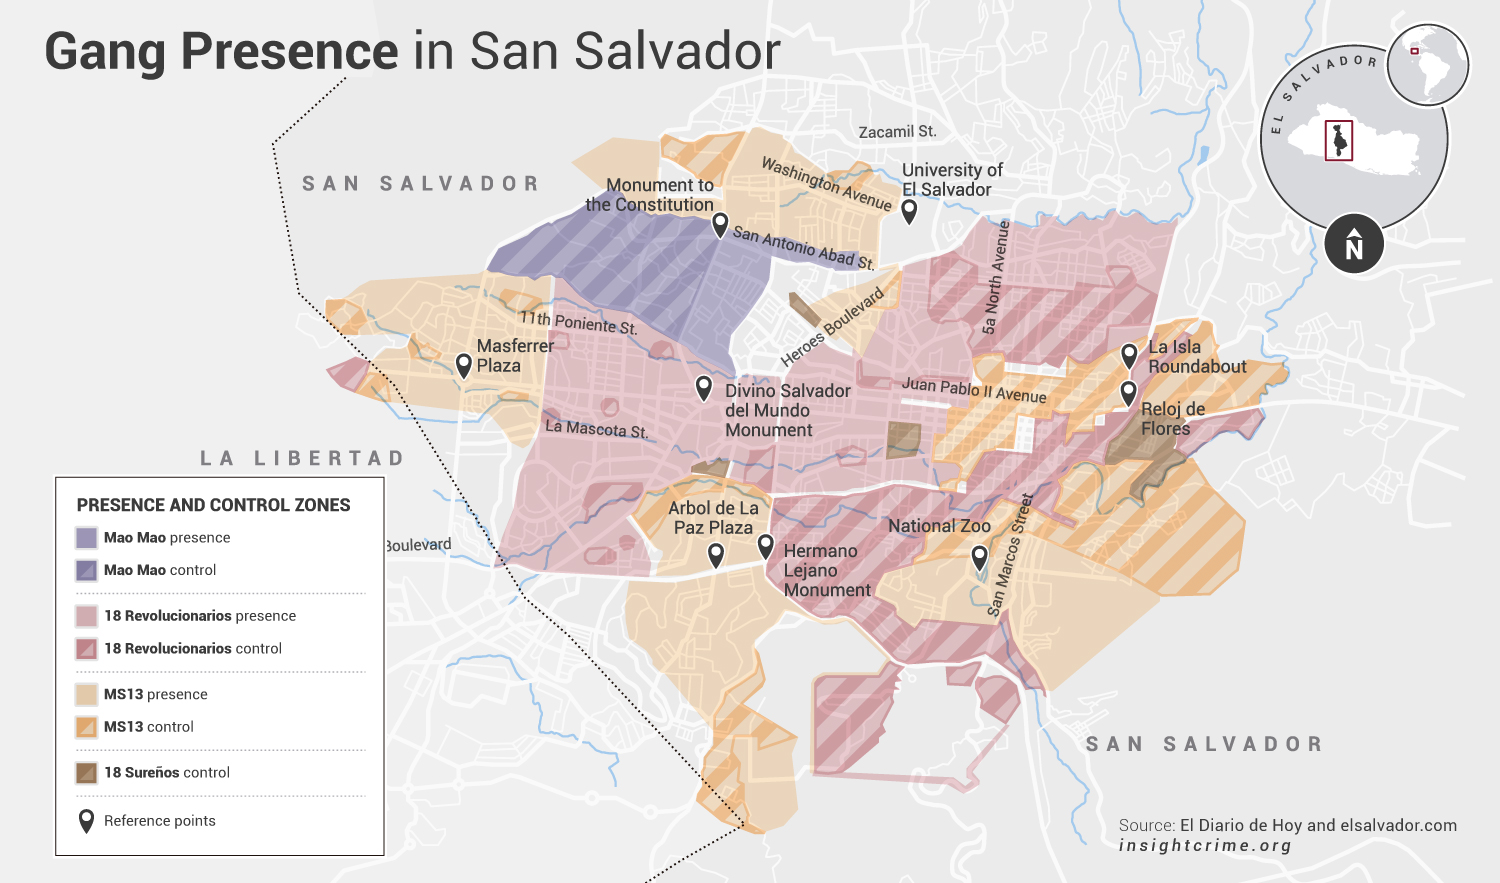
\includegraphics[width = \textwidth]{img/gangs_salvador}
%
% \end{frame}
% % ----------------------------------------------------

% ============================================================
% ============================================================
% NATIONALISM
% ============================================================
% ============================================================

\begin{frame}
\frametitle{Nations and Nationalism}
\centering

\begin{itemize}
  \item Rise of nationalism in the late 18th/early 19th centuries, and its relationship with political violence
  \item[]
  \item Nations: `imagined communities' of people with a sense of commonality based on linguistic, territorial, ethnic, or religious traits
  \item Nations $=$ fully mobilized ethnic groups, claims of statehood
  \begin{itemize}
    \item Some ethnic groups do not claim statehood, some nations are multi-ethnic (Switzerland)
  \end{itemize}
  \item Nationalism: political ideology, congruence between units of political sovereignty and nations
\end{itemize}

\end{frame}

\begin{frame}
\frametitle{Emergence of nationalism}
\centering

\begin{itemize}
  \item American Revolution
  \item Independence movements in Spanish South America
  \item French Revolution
  \item Full development during 19th century
\end{itemize}

\end{frame}

% \begin{frame}
% \frametitle{Why it happened}
% \centering
%
% \begin{itemize}[<+->]
%   \item Several theories explaining the rise of nationalism
%   \item Economic modernization (Ernest Gellner)
%   \begin{itemize}
%     \item Industrial revolution, homogenous workforce, standardized education
%   \end{itemize}
%   \item Rise of cultural modernization (Benedict Anderson)
%   \begin{itemize}
%     \item Mass literacy in vernacular languages, rise of printing press capitalism, legacies of administrative divisions
%   \end{itemize}
%   \item Shift to direct rule (Charles Tilly, Michael Hechter, etc)
%   \begin{itemize}
%     \item Homogenous state administration, nation-building policies, etc
%   \end{itemize}
%   \item Other theories: Meyer's world polity theory, ...
% \end{itemize}
%
% \end{frame}

\begin{frame}
\frametitle{The French Revolution and warfare}
\centering

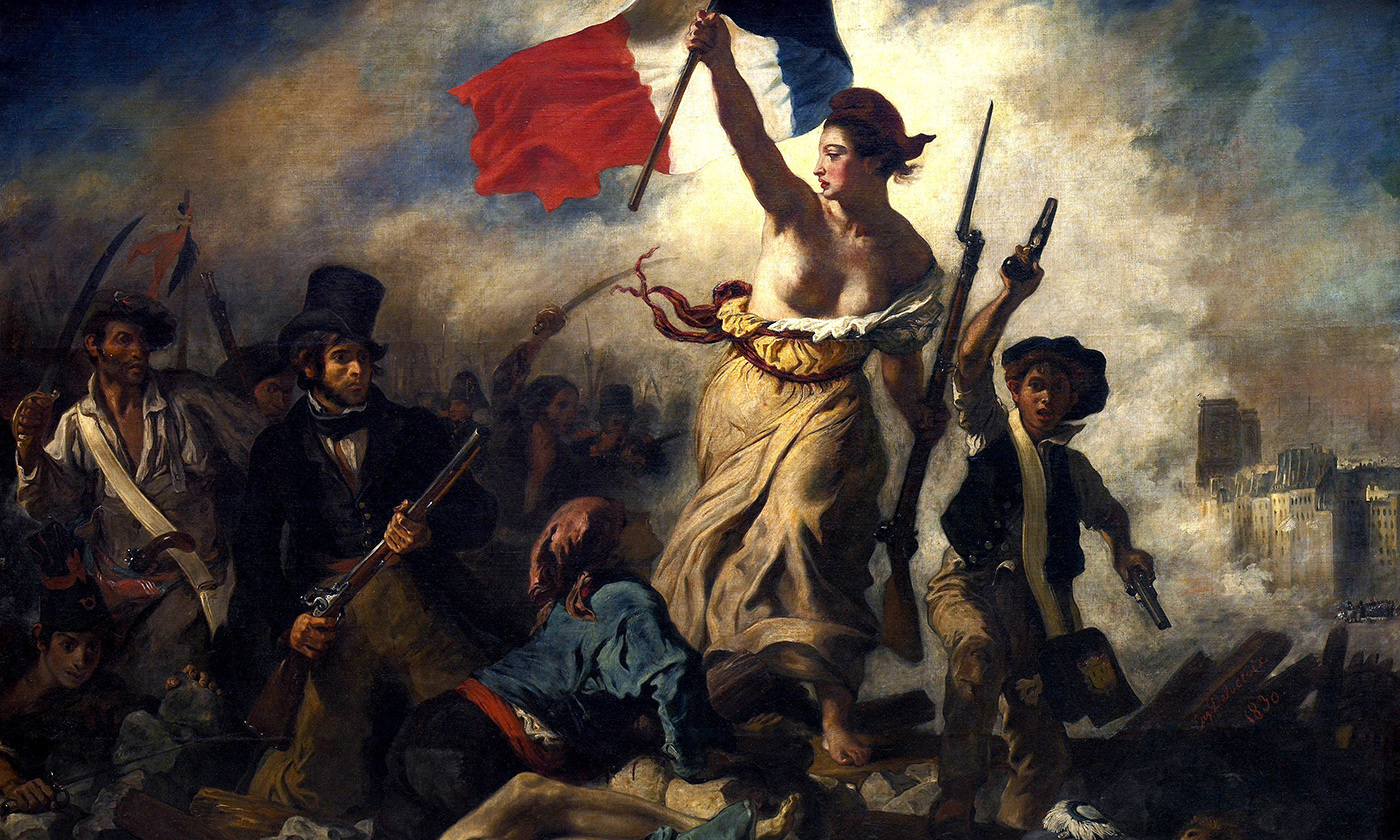
\includegraphics[width = 0.6\textwidth]{img/delacroix}

% Delacroix (1930)

\vspace{15pt}

\begin{quote}
  {\small ``in 1793 a force appeared that beggared all imagination. Suddenly war again became the business of the people---a people of thirty millions, all of whom considered themselves to be citizens. (...) the full weight of the nation was thrown into the balance.''}
\end{quote}

{\small (Clausewitz, \textit{On War})}

\end{frame}

\begin{frame}
\frametitle{What happened in international politics?}
\centering

\begin{itemize}
  \item Main idea: Nationalist systems change after French Revo
  \item Gilpin's typology of international change
  \begin{itemize}
    \item Interaction change (the way states relate to each other)
    \item Systemic change (`Waltzian' balance, etc)
    \item Systems change (the very \textit{nature} of the units)
  \end{itemize}
  \item Previous change: Westphalia and the territorial systems change
  \item Explaining impact on inter-state warfare at a global level
  \begin{itemize}
    \item \textit{historical} patterns of war
  \end{itemize}
  % \item[]<1-> {\footnotesize \textit{Source:} Cederman, Camber Warren, and Sornette (\textit{International Organization}, 2011)}
 \end{itemize}

\end{frame}

\begin{frame}
\frametitle{Territorial systems change}
\centering

\begin{itemize}
  \item Usual date: Peace of Westphalia in 1648
  \item Emergence of the modern state
  \item New scenario: internal monopoly of violence \& territorial sovereignty
  \item Direct, coercive methods of resource extraction
  \begin{itemize}
    \item Different from indirect rule, where tax/resource collection and coercion are outsourced
  \end{itemize}
  \item New warfare: Standing armies, better weapons, larger wars, ...
\end{itemize}

\end{frame}

\begin{frame}
\frametitle{Nationalist systems change}
\centering

\begin{itemize}
  \item Usual date: French Revolution
  \begin{itemize}
    \item Birth of the modern \textit{nation}, the imagined communities
  \end{itemize}
  \item New technology of statecraft: nation-building through mass schooling, mass mobilization, popular sovereignty, etc
  \begin{itemize}
    \item Remember previous technologies of statecraft: earliest states and the `domestication' of humans (Scott), Early Modern Europe and the emergence of direct rule (Tilly), etc
  \end{itemize}
  \item Loyalty replaces coercion, mass popular armies replace professionals
  \begin{itemize}
    \item That's why Clausewitz spoke of a new ``force ... that beggared all imagination'', and added that ``nothing now impeded the vigor with which war could be waged''
  \end{itemize}
\end{itemize}

\end{frame}

\begin{frame}
\frametitle{Did the French Revolution change warfare?}
\centering

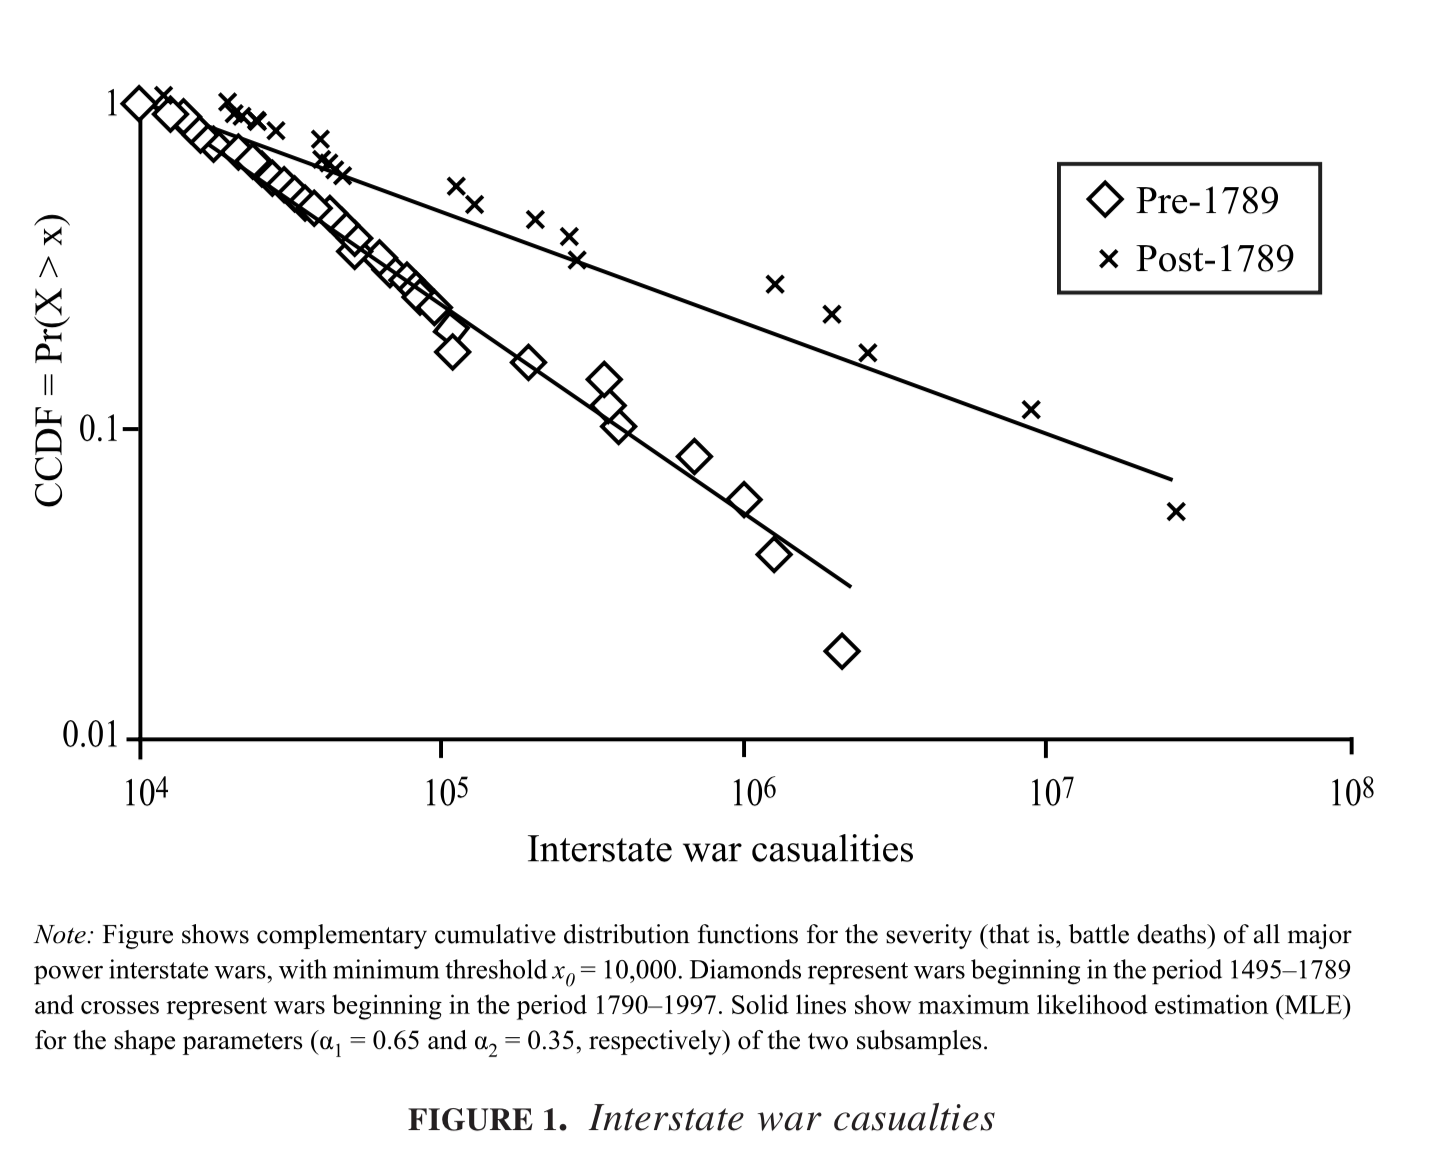
\includegraphics[width = 0.85\textwidth]{img/cederman_et_al_fig1}

{\scriptsize \textit{Source:} Cederman, Camber Warren, \& Sornette (2011)}

\end{frame}

\begin{frame}
\frametitle{Did the French Revolution change warfare?}
\centering

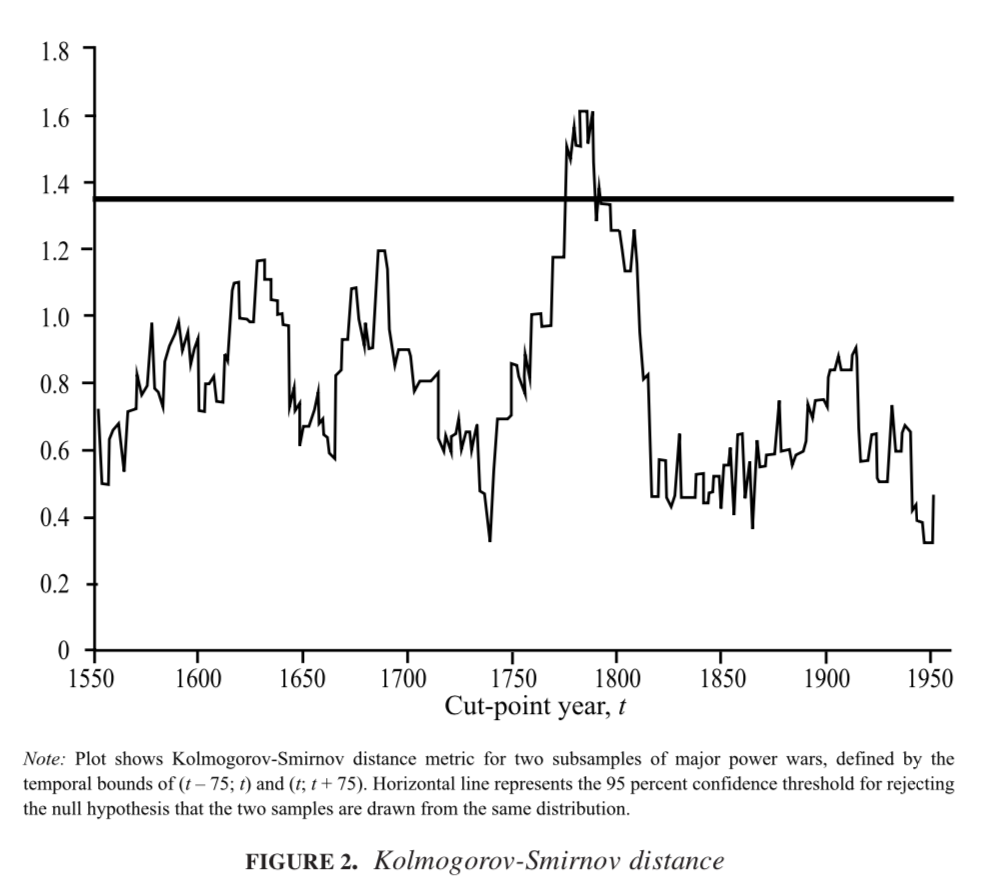
\includegraphics[width = 0.75\textwidth]{img/cederman_et_al_fig2}

{\scriptsize \textit{Source:} Cederman, Camber Warren, \& Sornette (2011)}

\end{frame}

\begin{frame}
\frametitle{Major institutional changes and war}
\centering

\begin{itemize}
  \item Usual studies of war occurrence focus on specific wars, and the conditions leading to each war onset
  \item \BGyellow{Global explanations for historical patterns of warfare} over the long run?
  \item Looking at how polities are organized and how they changed globally
  \item Claim: likelihood of wars (both interstate and civil wars) is higher in periods of institutional change, in particular, the main two processes taking place in the last 200 years: incorporation into empires and formation of nation-states
  % \item \textit{Source:} Wimmer \& Min (\textit{American Sociological Review}, 2006)
\end{itemize}

\end{frame}

\begin{frame}
\frametitle{Empires \& nation-states}
\centering

\begin{itemize}
  \item Two competing \BGyellow{models of state-building} since the French Rev
  \item Empires
  \begin{itemize}
    \item Centralized bureaucratic government, core region ruling over the periphery, claims to universal legitimacy (ideologies, religion), ...
  \end{itemize}
  \item Nation-states
  \begin{itemize}
    \item Also centralized bureaucracy, but uniform rule over a territory and claims to popular sovereignty
  \end{itemize}
  \item Displacing previous institutional set-ups: absolutist kingdoms, city states, feudalism...
\end{itemize}

\end{frame}

\begin{frame}
\frametitle{Empires \& nation-states}
\centering

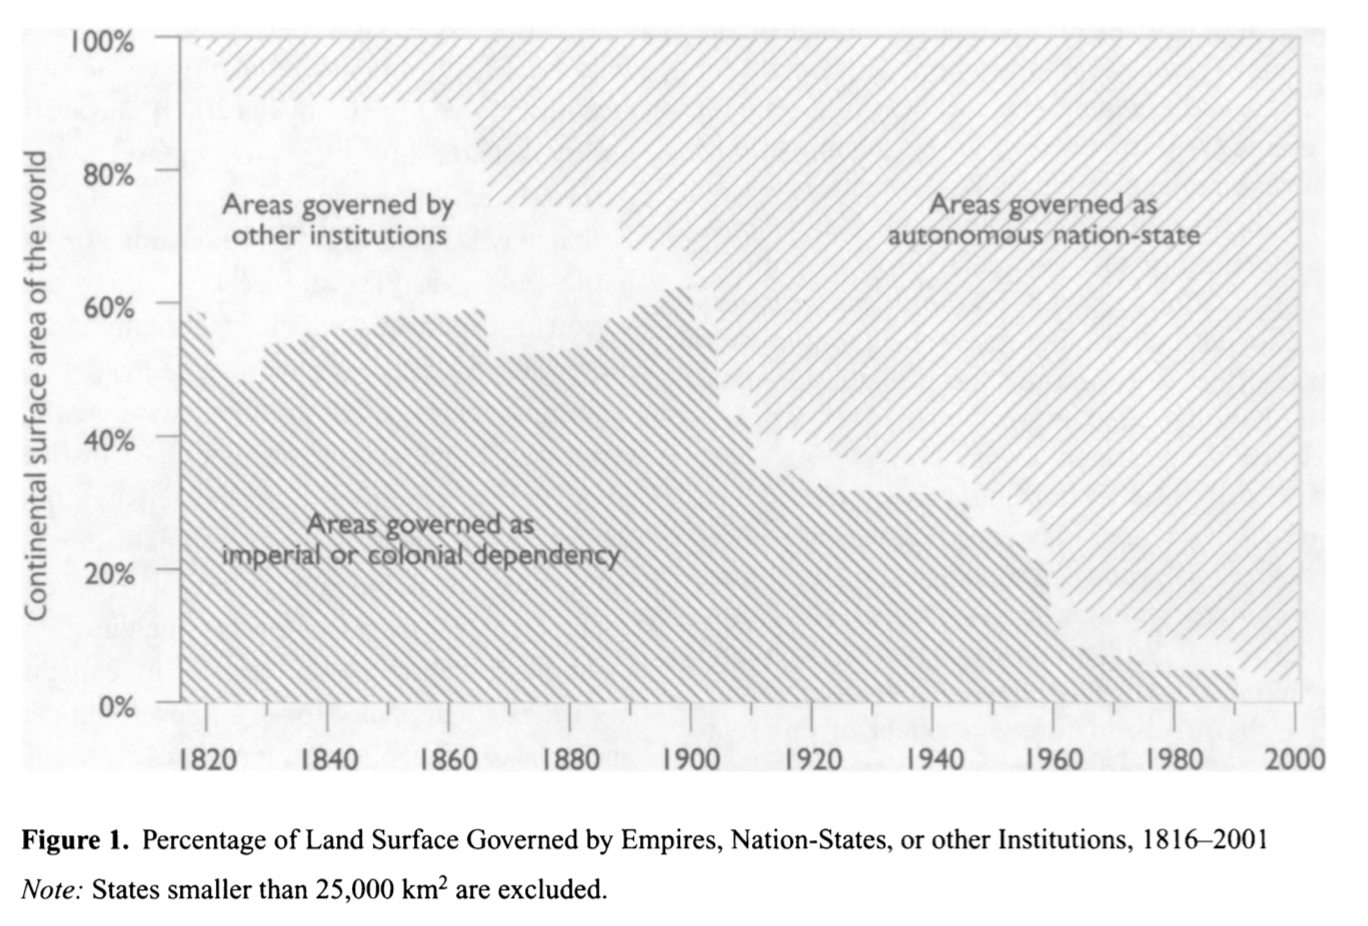
\includegraphics[width = \textwidth]{img/wimmer_min_fig1}

{\scriptsize \textit{Source:} Wimmen \& Min (2006)}

\end{frame}

\begin{frame}
\frametitle{Why war?}
\centering

\begin{itemize}
  \item \textit{Competing} models of state building
  \item Wars not because of changes to the international balance (as in Waltz), but because of \BGyellow{internal processes} and \BGyellow{competing claims to the same territory or population}
  \item Creating an empire will cause resistance to incorporation, particularly in the peripheries
  \item Formation of nation-states leads to the violently reordering of states (inter-state wars) or, once they are formed, wars over internal power distribution
\end{itemize}

\end{frame}


\begin{frame}
\frametitle{Institutional changes and wars}
\centering

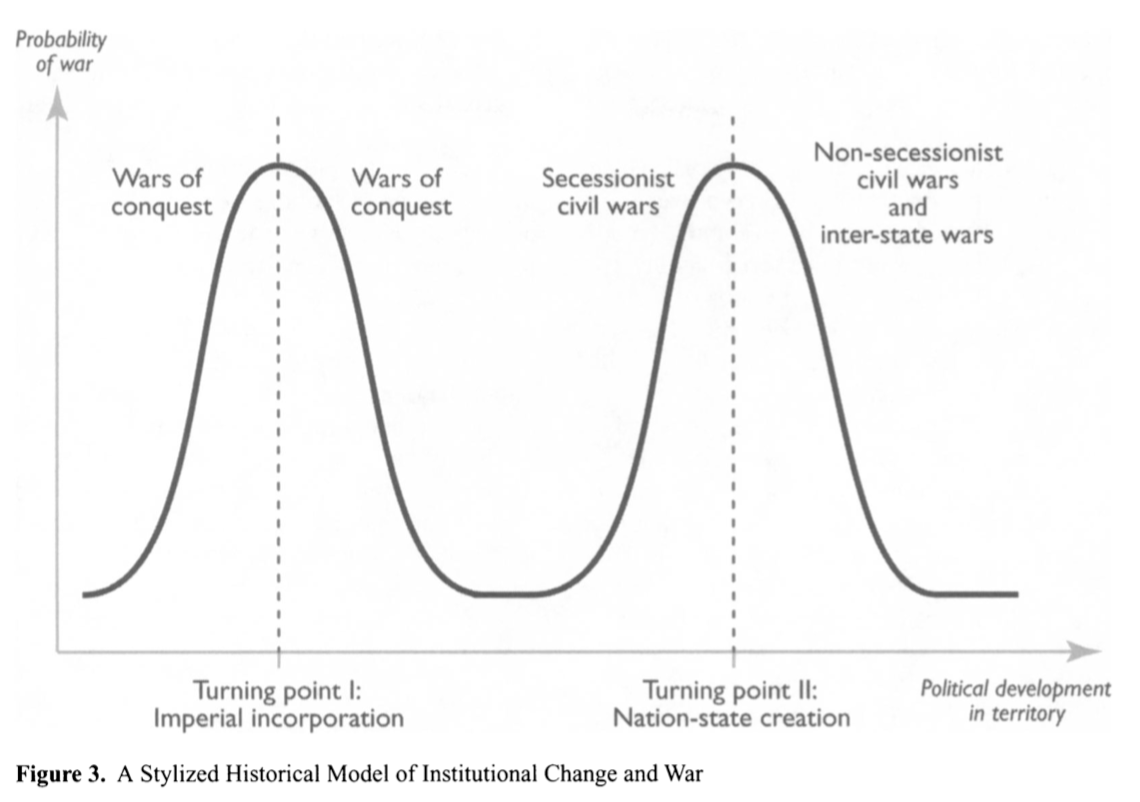
\includegraphics[width = 0.85\textwidth]{img/wimmer_min_fig3}

{\scriptsize \textit{Source:} Wimmen \& Min (2006)}

\end{frame}

\begin{frame}
\frametitle{Nation-states and wars}
\centering

\begin{itemize}[<+->]
  \item The rise of nationalism and nation-states in the world linked to different types of war
  \item Creating a nation-state often involves splitting off from a former polity: \BGyellow{secessionist wars}
  \begin{itemize}
    \item Many conflicts throughout the world (e.g. ETA in Spain)
  \end{itemize}
  \item Congruence between nations and states (nationalism) leads to \BGyellow{irredentism wars}
  \begin{itemize}
    \item Irredentism: from Italian \textit{irredento} (unredeemed), about territories inhabited by Italian-speaking populations ruled by the Austro-Hungarian empire during the 19th century
    \item E.g.: Ireland and Ulster, Nagorno-Karabakh?
  \end{itemize}
  \item Once nation-states are formed, conflicts over the distribution of power, ethno-political discrimination (\BGyellow{civil wars})
\end{itemize}

\end{frame}

\begin{frame}
\frametitle{Nation-states and wars}
\centering

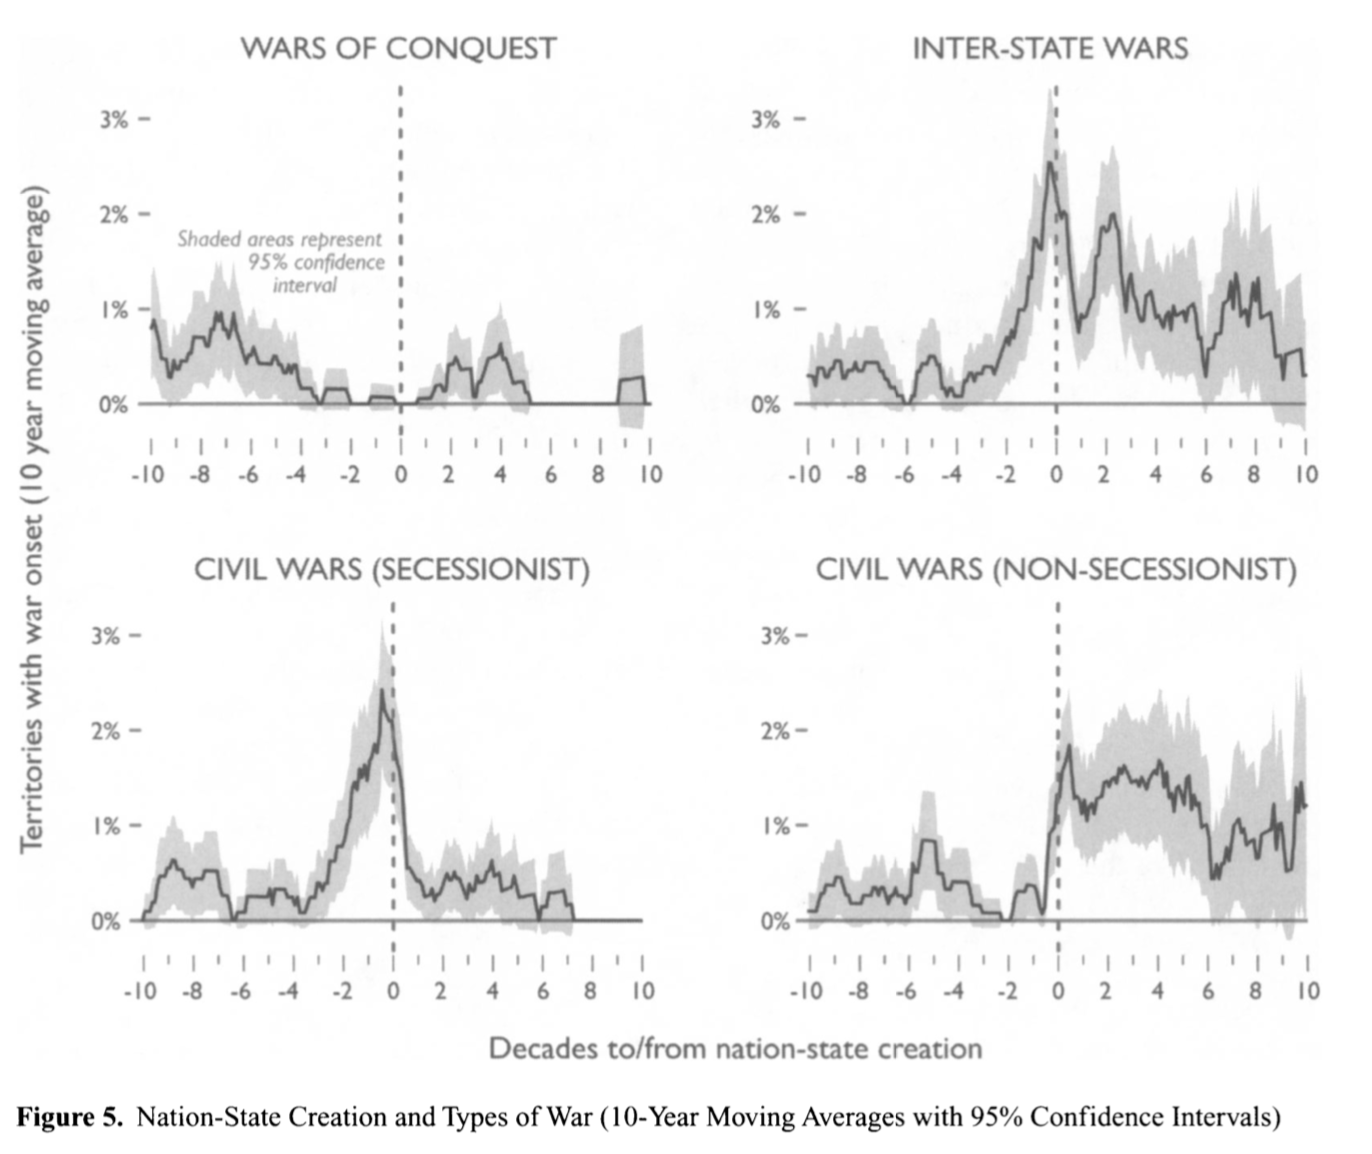
\includegraphics[width = 0.75\textwidth]{img/wimmer_min_fig5}

{\scriptsize \textit{Source:} Wimmen \& Min (2006)}

\end{frame}
% ----------------------------------------------------

% % ----------------------------------------------------
% \begin{frame}
% \frametitle{Looking at the big picture}
% \centering
%
% \begin{itemize}
%   \item Different type of questions:
%   \begin{itemize}
%     \item How did warfare evolve? How do changes to the international system impact overall levels of war?
%   \end{itemize}
%   \item $\neq$ explanations of political conflicts in particular
%   \begin{itemize}
%     \item explain the outbreak of individual conflicts, assess likelihood of a conflict in a given country
%   \end{itemize}
%   \item But these are macro-historical explanations: focus is on the evolution of warfare throughout history and what macro-level changes explain it
%   \item Related to previous lecture on warfare and state formation
% \end{itemize}
%
% \end{frame}
% % ----------------------------------------------------

% % ----------------------------------------------------
% \begin{frame}
% \frametitle{Nationalism and internal conflict}
% \centering
%
% \begin{itemize}[<+->]
%   \item Different perspective on nationalism and war: how it impacts specific internal conflicts
%   \item Ethnicity $\neq$ nationalism
%   \begin{itemize}
%     \item Closely related concepts, sometimes (especially years ago) treated very differently
%     \item Difference: claims of statehood (multi-ethnic nations, civic vs. ethnic nationalism, etc)
%   \end{itemize}
%   \item Early studies on ethnic conflict
%   \begin{itemize}
%     \item Almost no attention to the state, ethnic wars were seen as a conflict \textit{between} ethnic groups
%     \item Ancient hatred idea, security dilemma, etc
%   \end{itemize}
% \end{itemize}
%
% \end{frame}
% % ----------------------------------------------------
%
% % ----------------------------------------------------
% \begin{frame}
% \frametitle{Nationalism and internal conflict}
% \centering
%
% \begin{itemize}[<+->]
%   \item Modern studies put emphasis on the role of state and political power
%   \item Quantiative studies: role of grievances and ethnopolitical discrimination, etc (will see more on civil wars)
%   \item External conflict: nation-to-state deficit and surplus
%   \begin{itemize}
%     \item If nations and states match, political stability
%     \item State deficit: secessionist wars, etc
%     \item Nation deficit: irredentism
%     \item `Macedonian syndrome:' how nation-building spills off state borders and radicalizes host states, ethnic minorities, and irredentist states
%   \end{itemize}
%   \item Difference with previous macro-historical approach: looking at specific cases
% \end{itemize}
%
% \end{frame}
% % ----------------------------------------------------

\begin{frame}
\frametitle{Making up the nation through violence}
\centering

\begin{itemize}
  \item An ultimate version of the nation-to-state congruence: using violence to \textbf{make up the nation}
  \item Homogenizing policies: many available tools or strategies
  \item A last resort: ethnic cleansing or genocide
  \item Essentially a modern phenomenon, not about ancient barbarism
  \item Zygmunt Bauman's \textit{Modernity and Holocaust}
  % \item bulutgil etc
\end{itemize}

\end{frame}
% ----------------------------------------------------


% ----------------------------------------------------
\begin{frame}
\frametitle{Tomorrow's seminar}
\centering

\begin{itemize}
  \item `The birth of a new Ukraine': how Russia's war united a nation
  \item[]
  \item[-] Relationship between nationalism and war, macro-level
  \item[-] Role of national ID in fighting a war
  \item[-] Legitimacy: state and nation
  \item[-] What effect do wars have...
  \begin{itemize}
    \item[1.] in terms of state-building?
    \item[2.] internal national identification?
    \item[3.] nationalism in third-parties?
  \end{itemize}
\end{itemize}

\end{frame}
% ----------------------------------------------------


\end{document}
